\chapter{Results}

About the final program results

There ar not just things to finish or implement, also, it is nedded to solve some actual problems. Most important of them are:

Signal Path glitch and page switching.................................

Less important, are: ......................................................

\begin{itemize}
	\item \textbf{Filter Algorithms:}
	
	\item \textbf{User Limitations:} For example, since we are using the Sounddevice library and managing both inputs as a single input stream, we have the limitation that both channels must come from the same sound card. However, the program currently allows the selection of different sound cards for each input channel.
	
\end{itemize}

\section{Final tests}

For the final test, which involved a real-world scenario, I had the privilege of accessing professional equipment and a real theater. The venue was the \textbf{Teatre del Coro}, located in Sentmenat, Spain, and managed by the non-profit cultural association \textit{Societat Coral Obrera la Gloria Sentmenatenca}. The equipment available for the test was:

\begin{itemize}
	\item \textbf{EVO 4:} External USB audio interface, used as the sound card for the program.
	\item \textbf{Audix TM1:} Measurement microphone, used as the source for the \textbf{Input from System} signal.
	\item \textbf{Mackie SRM-750:} Loudspeaker, responsible for playing the \textbf{Output to System} signal.
	\item \textbf{External Laptop:} Device used to generate the \textbf{External Input} signal.
	\item \textbf{Behringer X32 Compact:} The theater's digital mixing console. It is required to route signals to the speaker. Since it is part of the system, it will also be used to compare the analysis tools of the RTA+C program with the built-in tools of the mixer.
\end{itemize}

The sound card and the measurement microphone were kindly provided by \textit{IMESDE, Integració, Distribució i Enginyeria Escènica, S.L.}, a private company located in La Garriga, Spain. All the devices used can be seen in Figure~\ref{fig:Coro_setup}.

The first step was to place the measurement microphone. It was important to choose a good position where the microphone could capture the sound from a single representative point in the room. The first parameter to define was the microphone height. This venue is very versatile throughout the week, and the seats can be removed. However, events held without the seats typically do not require the use of the theater's sound system. Therefore, it was more appropriate to take measurements with the seats in place. Unfortunately, on the day I was able to perform the measurements, the seats had been partially removed. Nevertheless, I positioned the microphone at the average height of a seated person, as shown in Figure~\ref{fig:Mic_pos1} and Figure~\ref{fig:Mic_pos2}.

\begin{figure}[H]
	\centering
	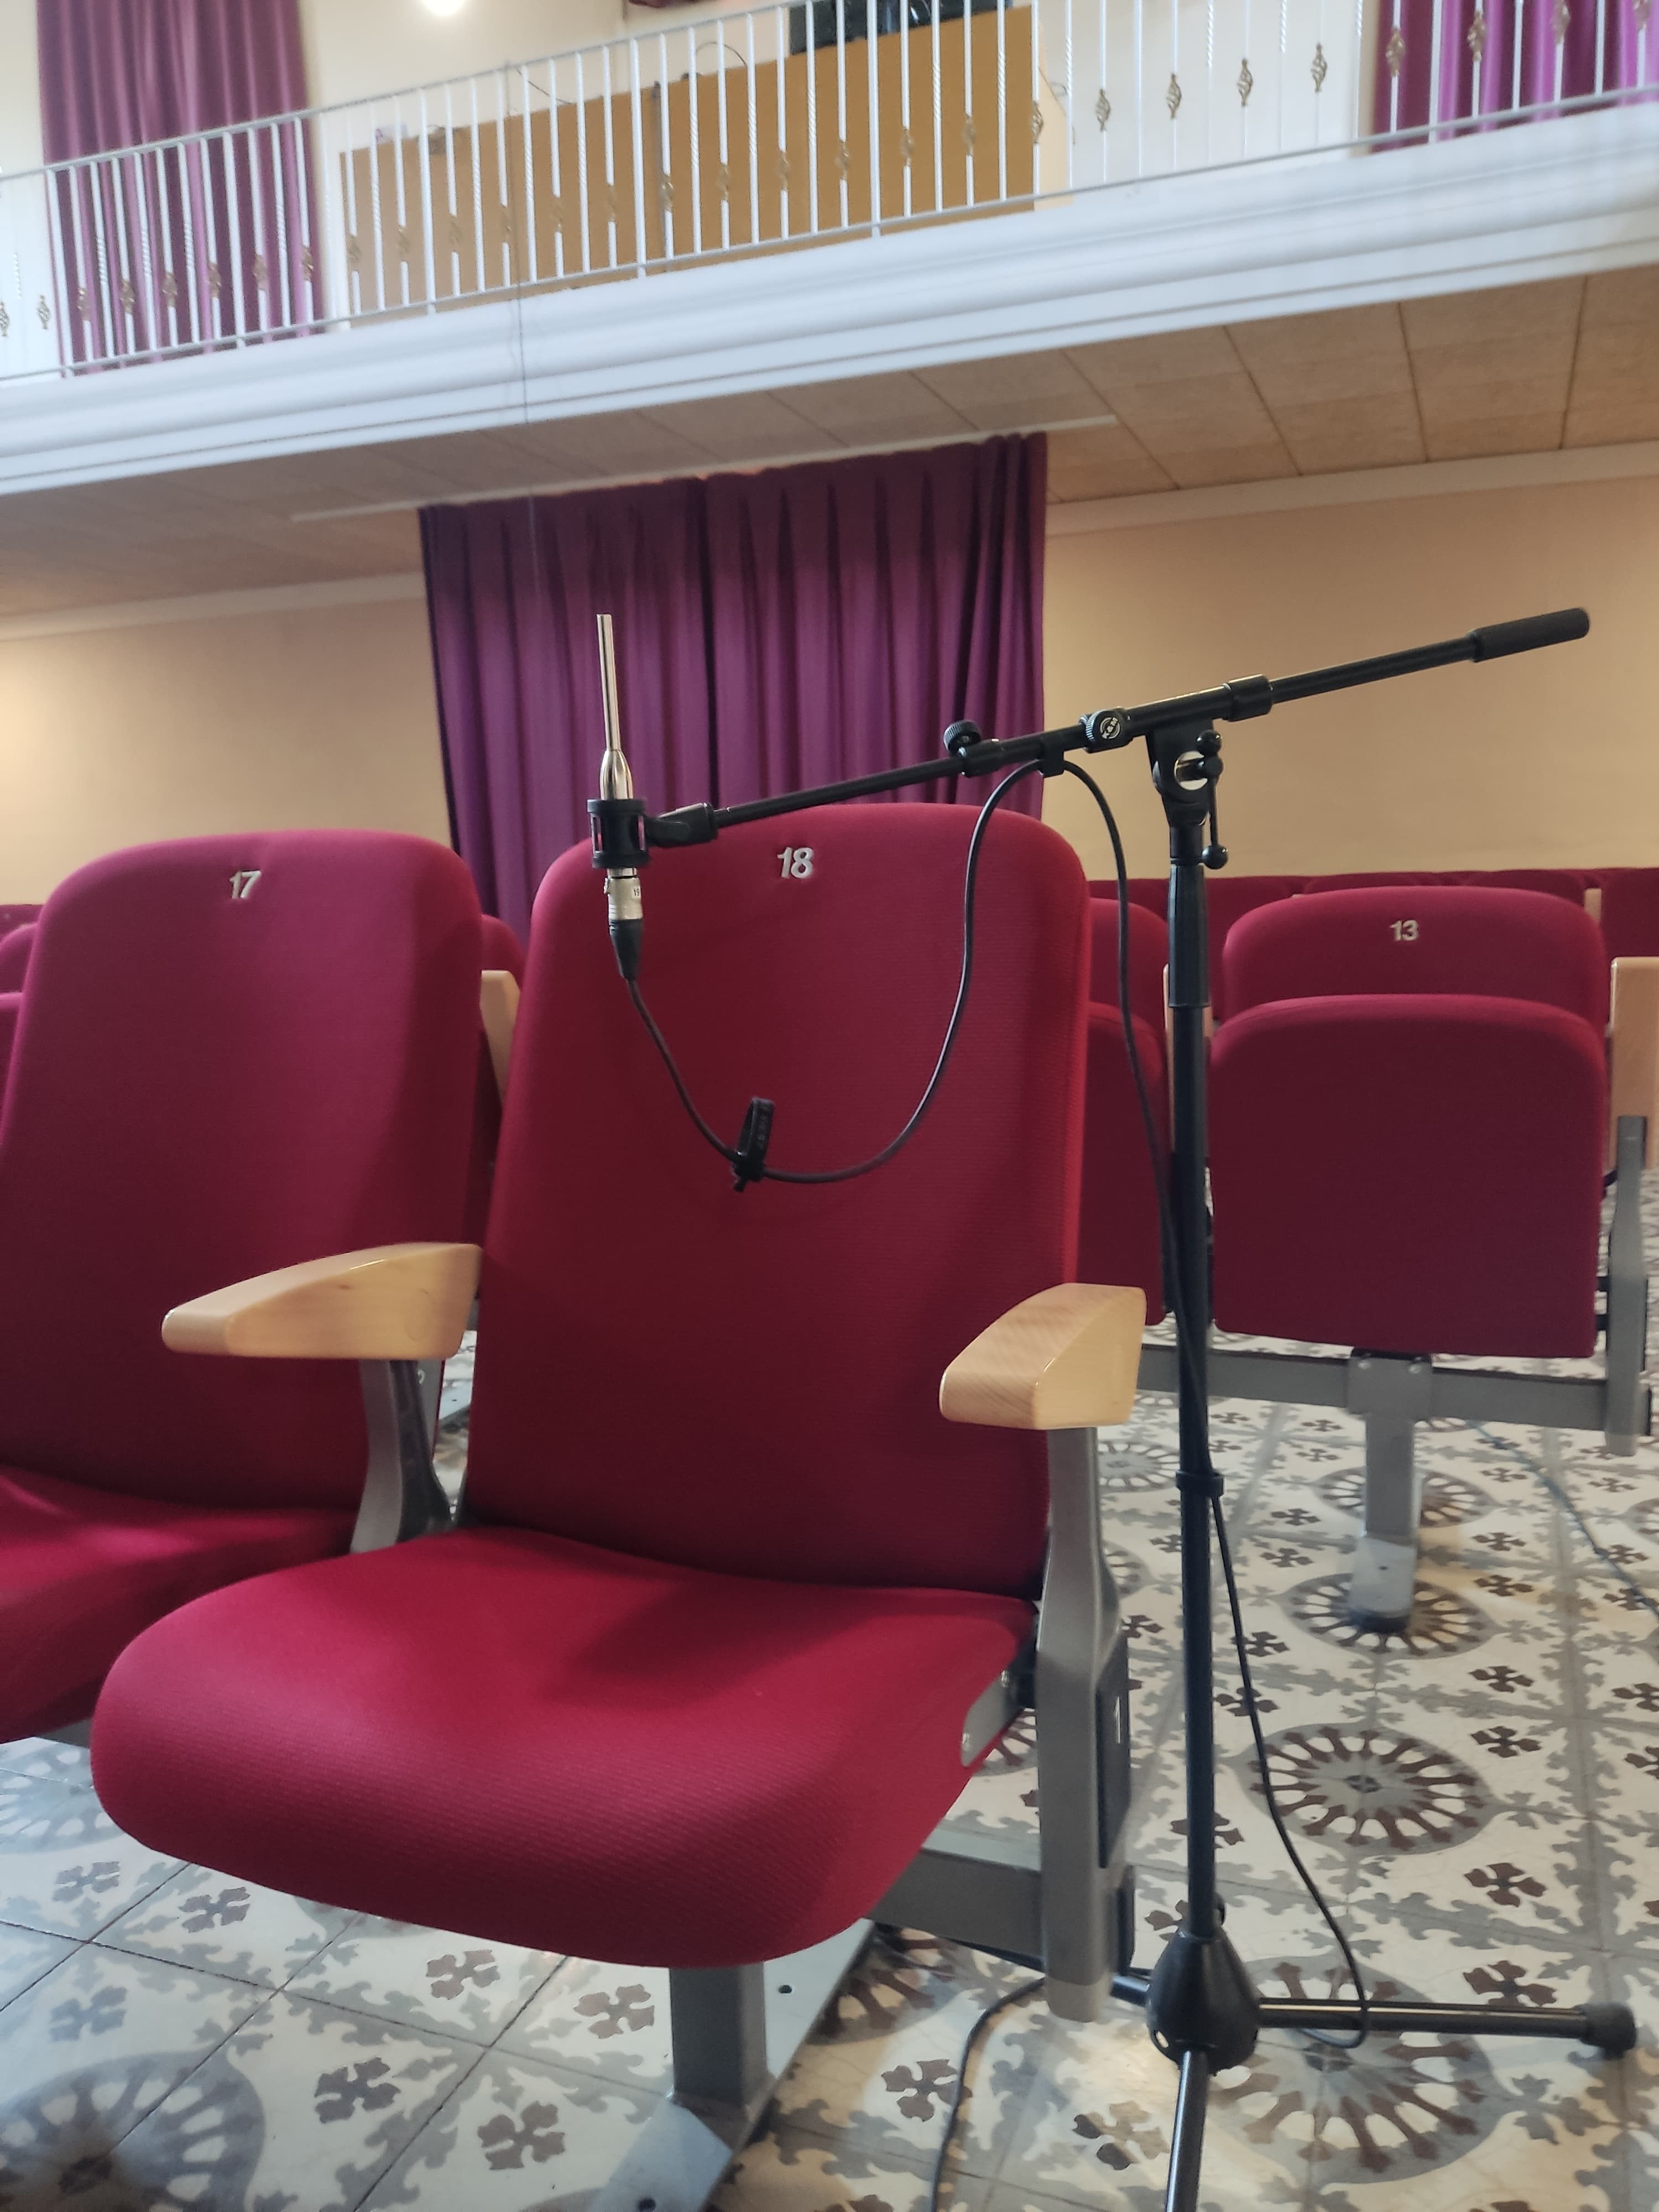
\includegraphics[width=0.6
	\linewidth]{Figures/Coro_micpos1.jpeg}
	\caption{Microphone height relative to the seat}
	\label{fig:Mic_pos1}
\end{figure}

\begin{figure}[H]
	\centering
	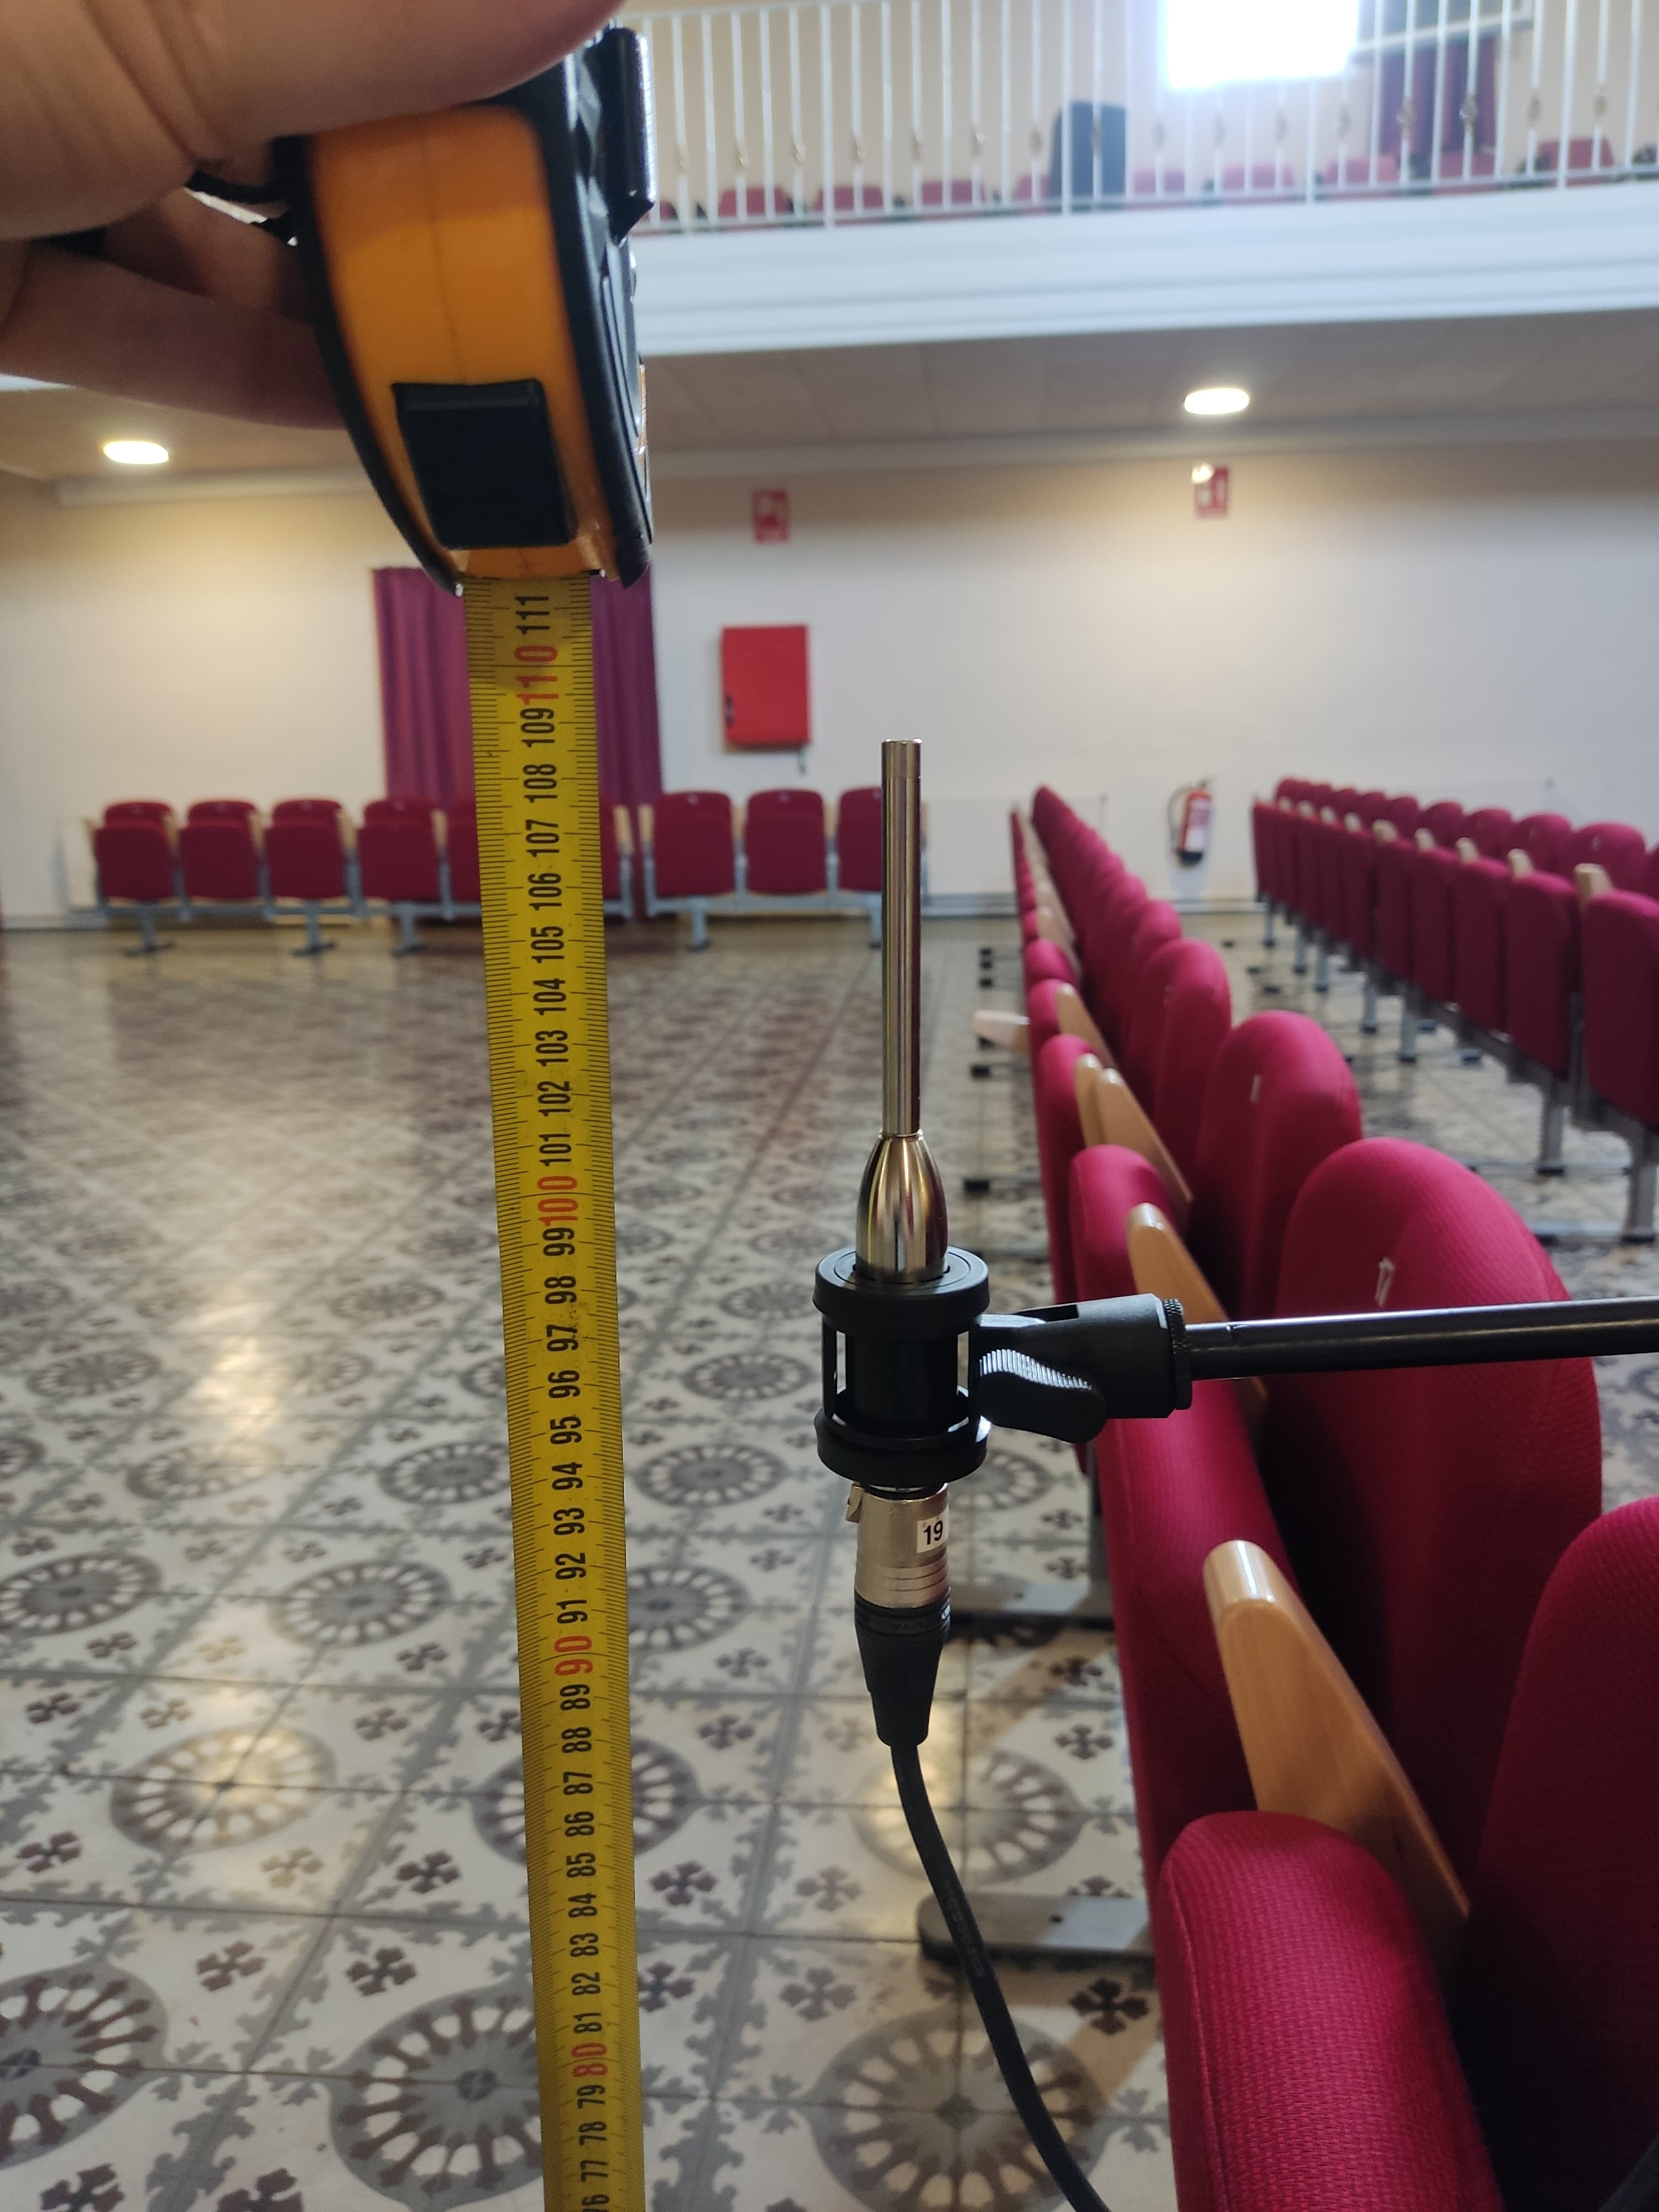
\includegraphics[width=0.6
	\linewidth]{Figures/Coro_micpos2.jpeg}
	\caption{Microphone height = 1.1m}
	\label{fig:Mic_pos2}
\end{figure}

Next, the microphone had to be placed at a representative point in the room. Since I was measuring only one speaker and the program operates in mono, the position had to be one where the speaker had good coverage and where the microphone was as close as possible to the center of the audience area. I decided to place the microphone approximately halfway through the depth of the room. Starting from a position where the speaker was directly in front of the microphone, I shifted it slightly to the right to bring it closer to the actual center of the room. As shown on figure~\ref{fig:Mic_pos3} and figure~\ref{fig:Floor_section}.
\begin{figure}[H]
	\centering
	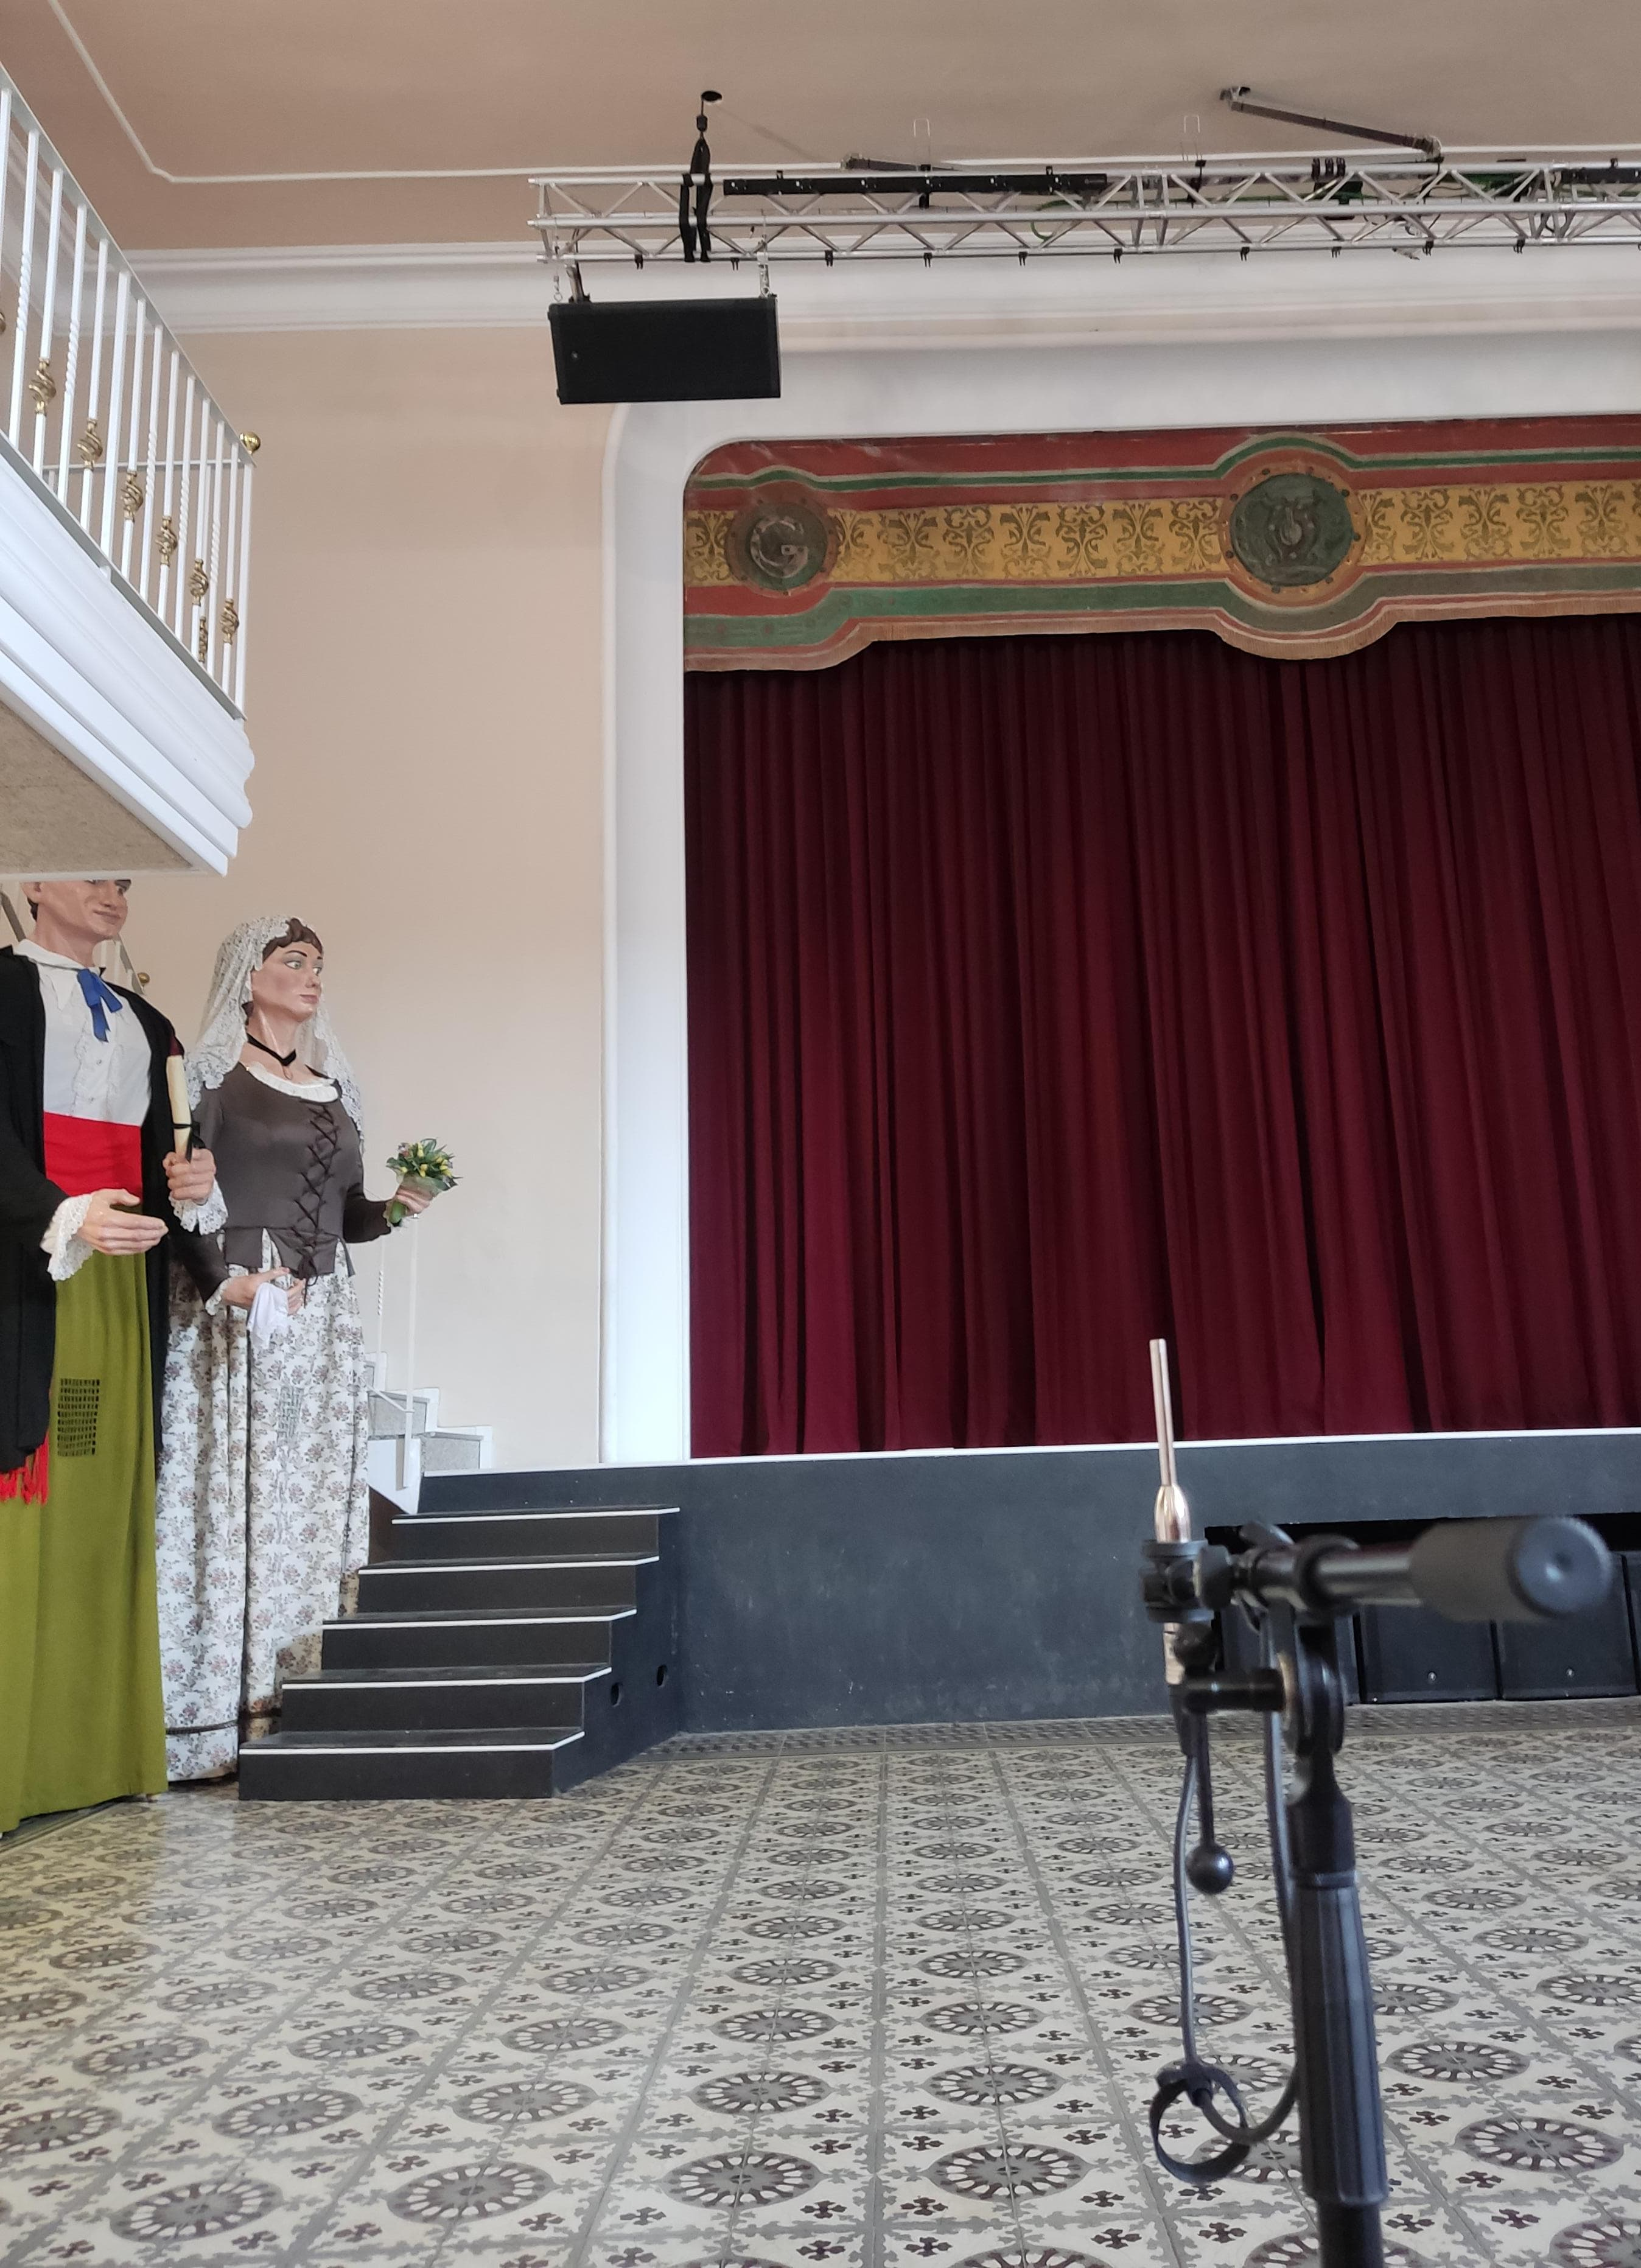
\includegraphics[width=0.6
	\linewidth]{Figures/Coro_micpos3.jpeg}
	\caption{Microphone position relative to the speaker}
	\label{fig:Mic_pos3}
\end{figure}

\begin{figure}[H]
	\centering
	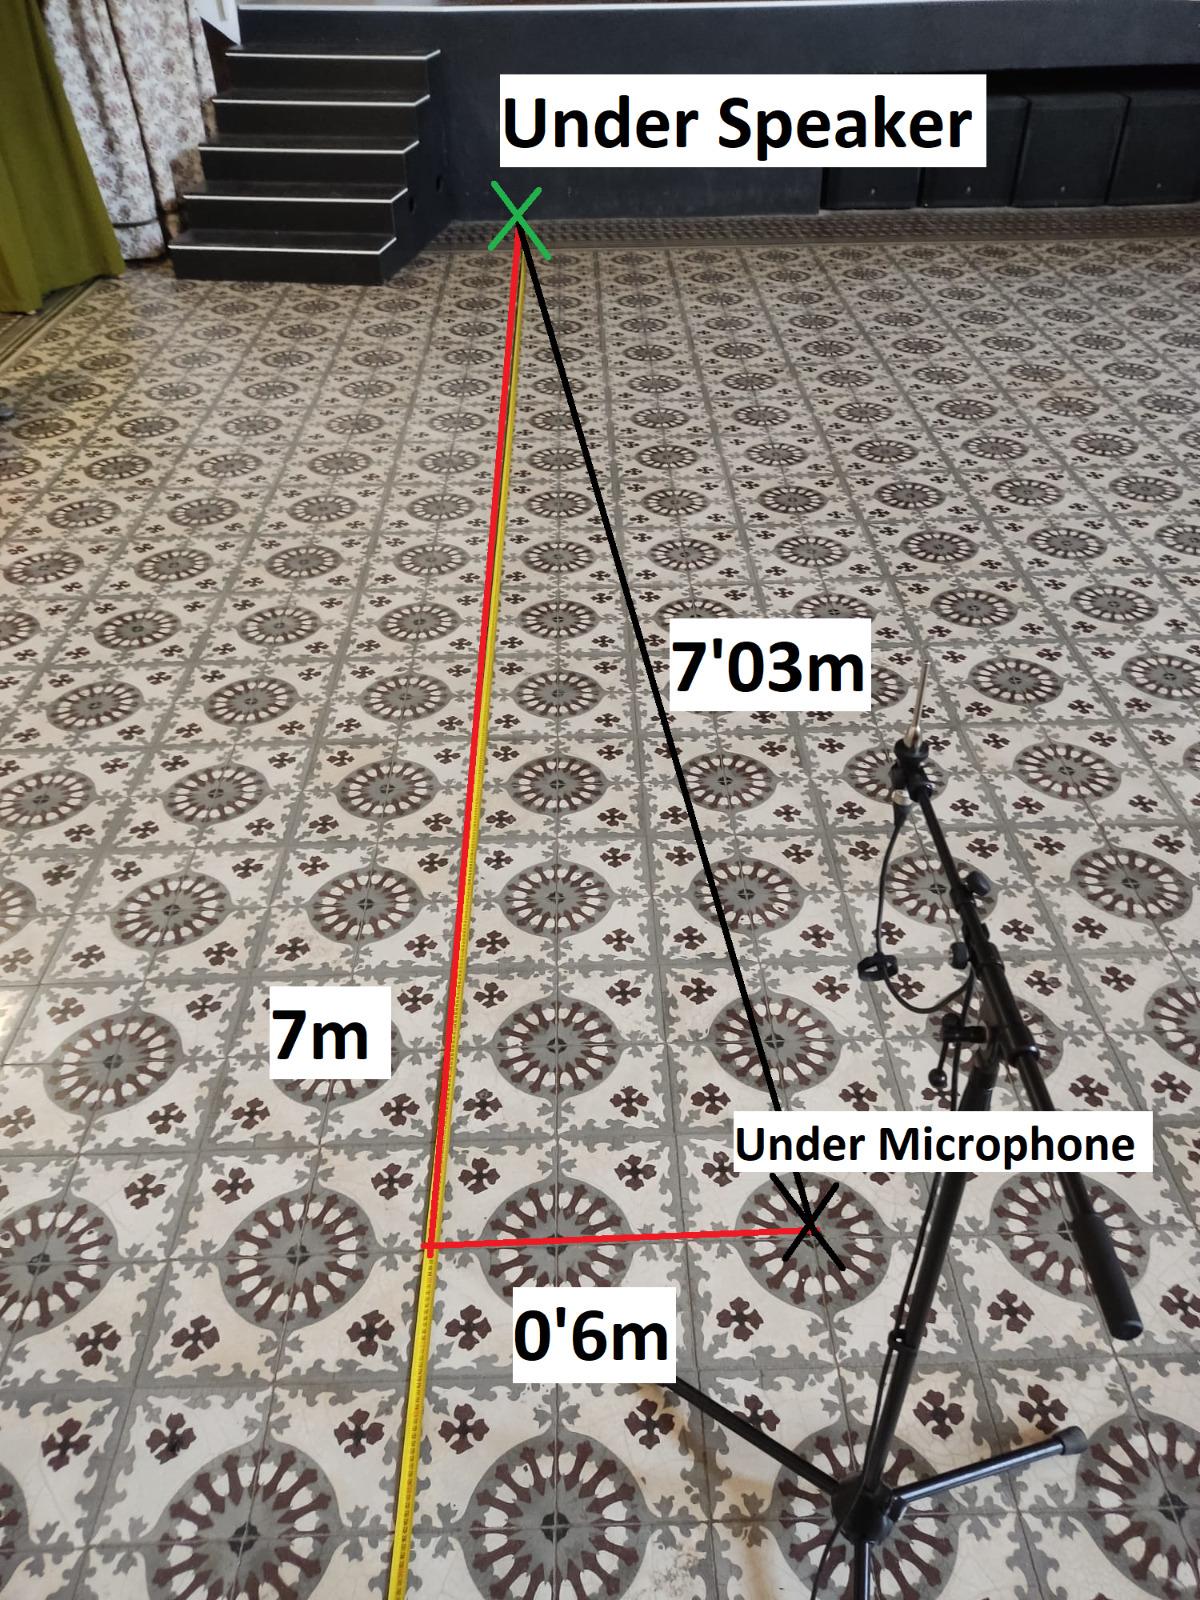
\includegraphics[width=0.6
	\linewidth]{Figures/Coro_floor_trigo.jpeg}
	\caption{Horizontal distance between speaker and microphone}
	\label{fig:Floor_section}
\end{figure}

Knowing that the speaker is suspended from a rigging bar at a hieght of approximately 6.5 m, and substrating the microphone height, the vertical distance between the two is around 5.4 m. Additionally, the horizontal distance—shown in Figure~\ref{fig:Floor_section}—is 7.03 m. Using basic trigonometric calculations, we can determine that the total distance between the speaker and the microphone is approximately 8.86 m, as illustrated in Figure~\ref{fig:spk-mic}.


\begin{figure}[H]
	\centering
	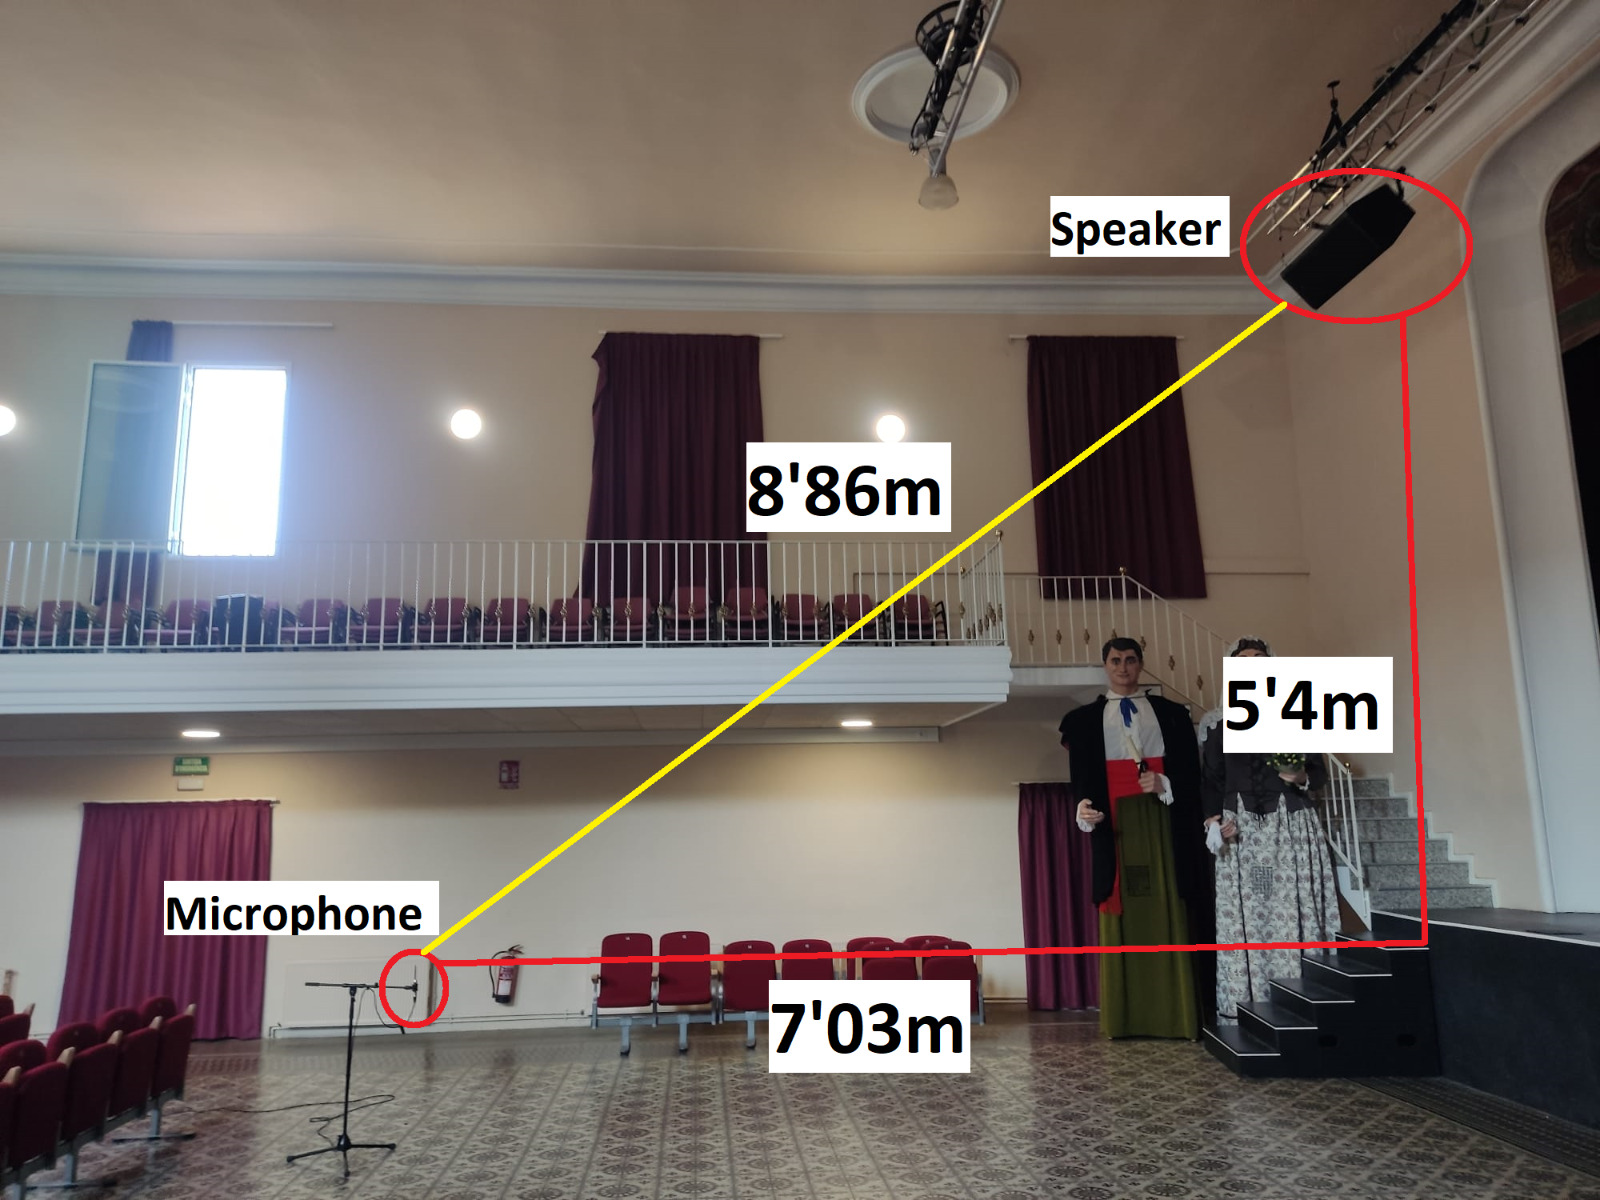
\includegraphics[width=1
	\linewidth]{Figures/Coro_section_trigo.jpeg}
	\caption{Distance between microphone and speaker}
	\label{fig:spk-mic}
\end{figure}

Once the microphone was positioned, it was time to set up the rest of the equipment, as shown in Figure~\ref{fig:Coro_setup}.

\begin{figure}[H]
	\centering
	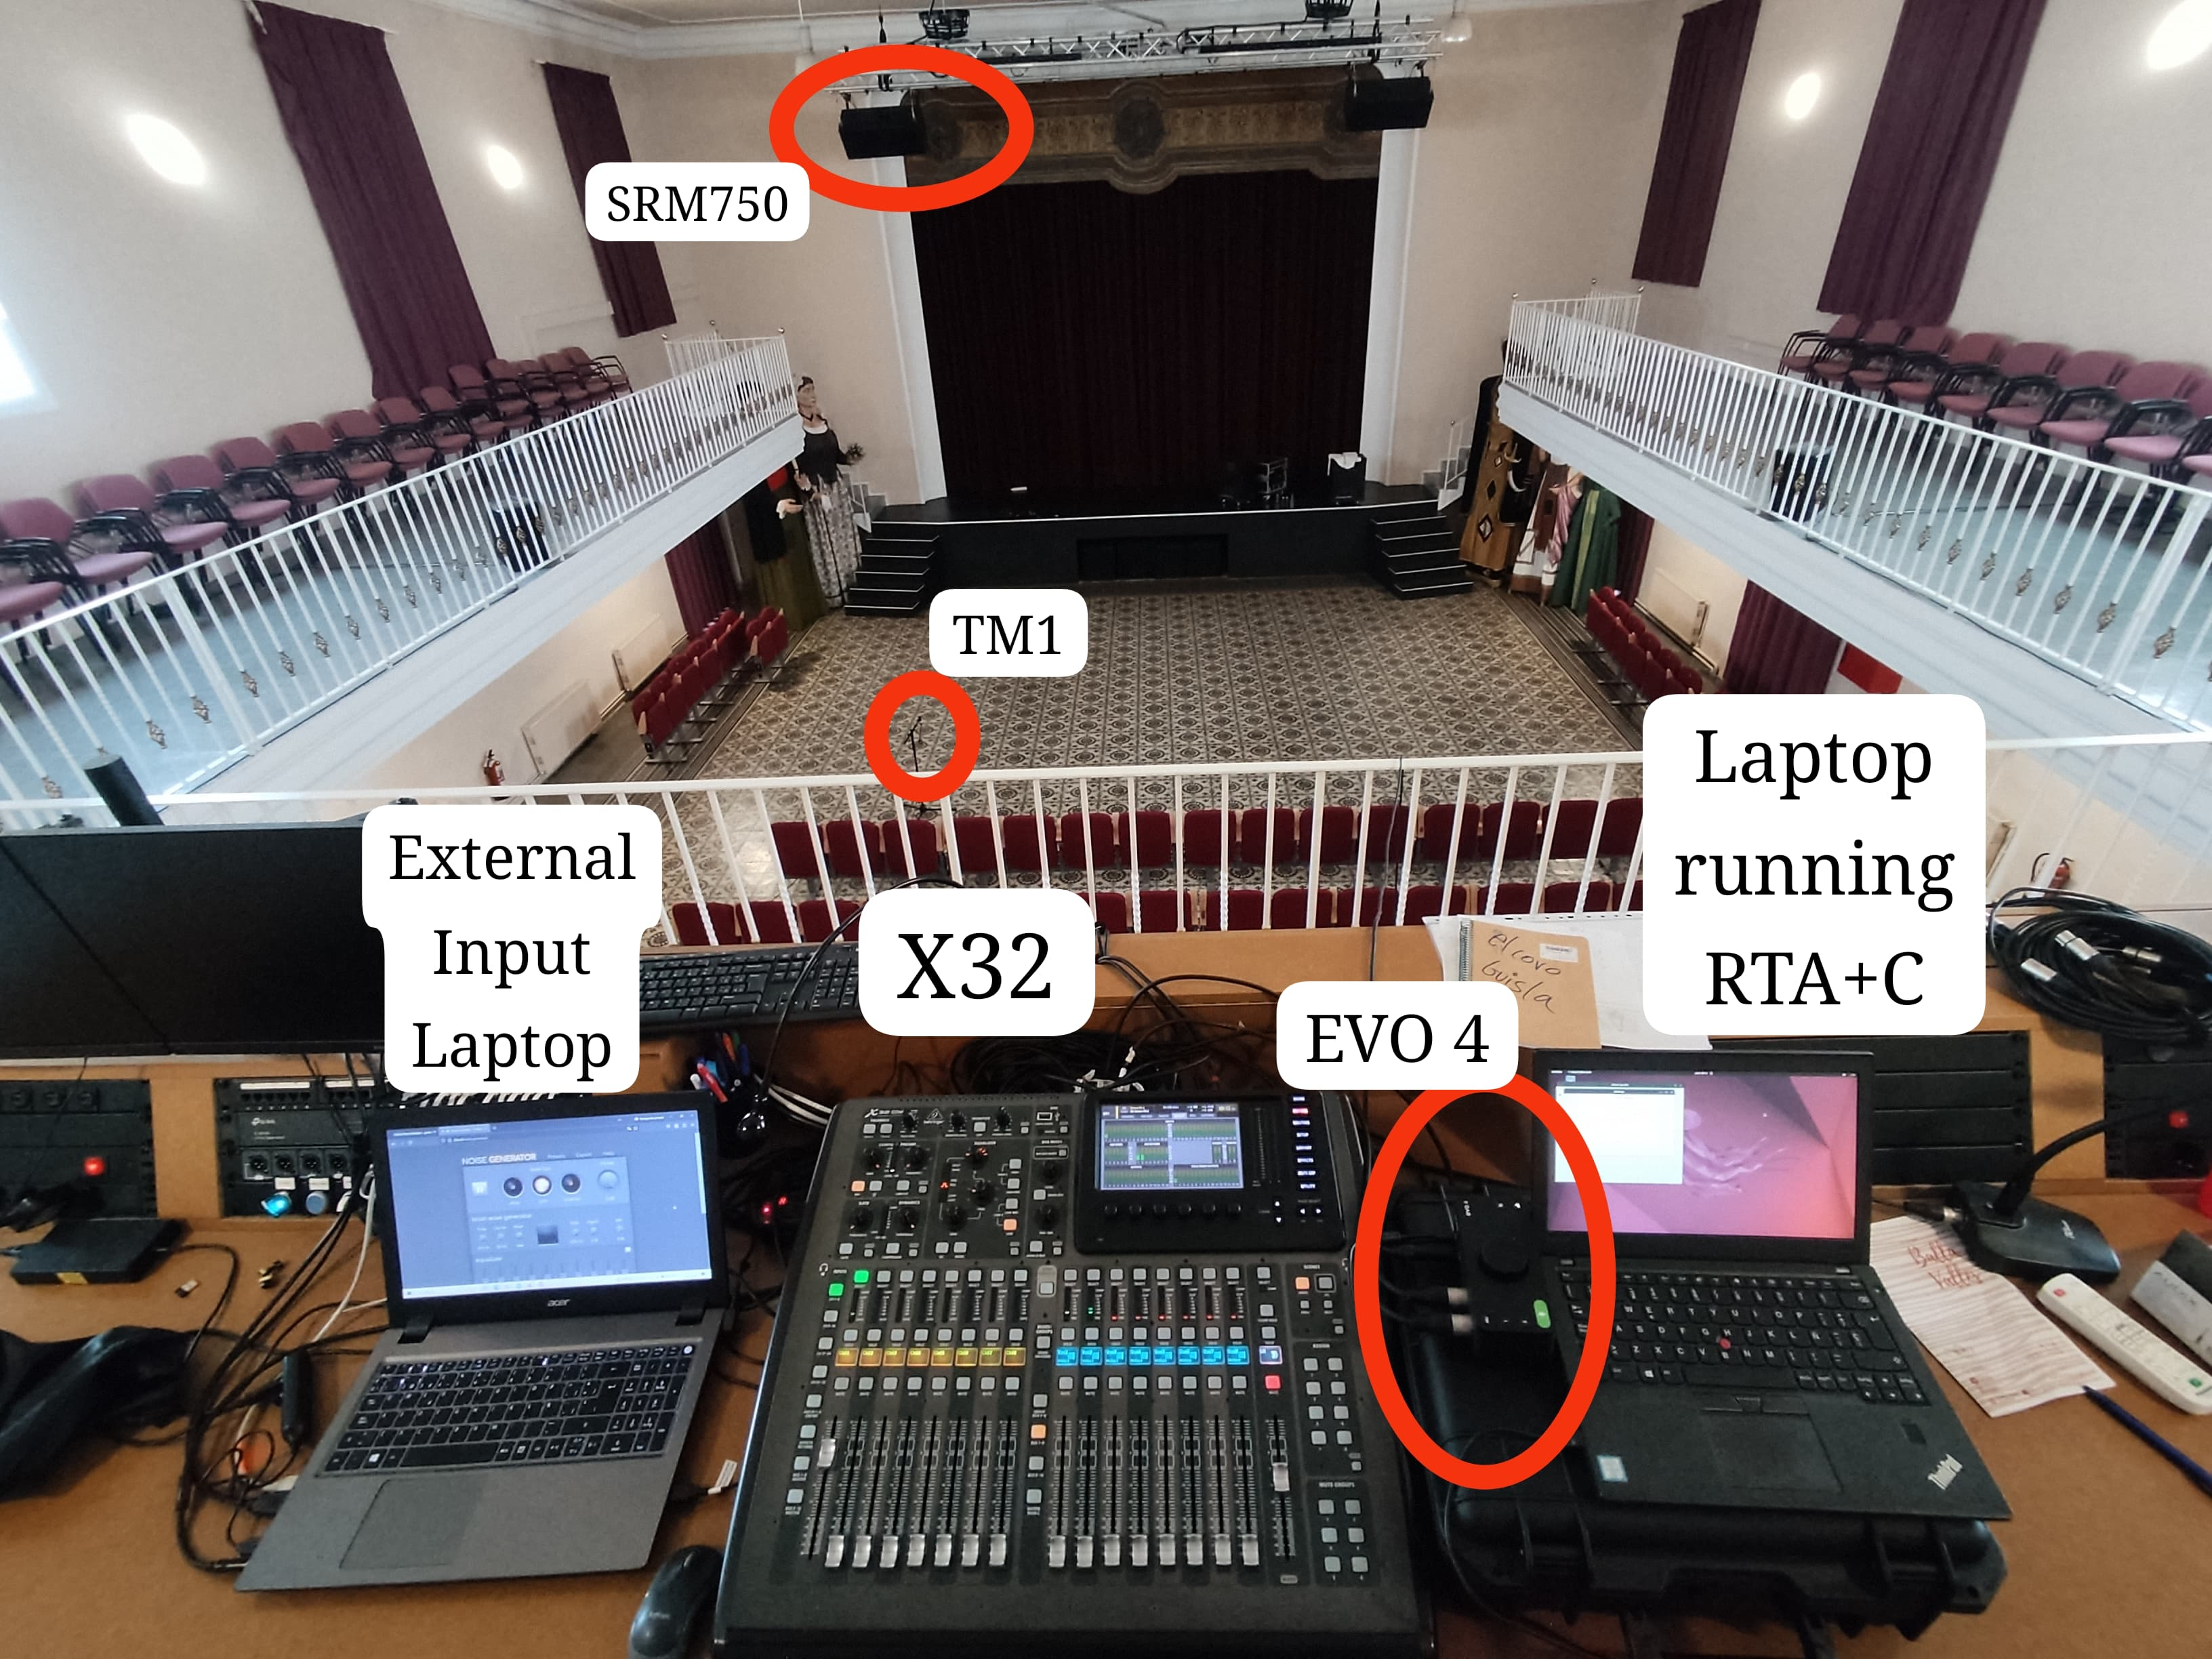
\includegraphics[width=1
	\linewidth]{Figures/Coro_setup.jpeg}
	\caption{All equipment set up}
	\label{fig:Coro_setup}
\end{figure}

In order to enable comparison between our software solution and the built-in tools of the digital mixing console (\textit{X32}), all signals must be routed through the \textit{X32}, as it offers advanced routing and distribution capabilities. Additionally, the console must be properly configured to route the signals correctly. Remember that we are using the \textit{EVO 4} as the audio interface for the RTA+C software, as shown in the following connection diagram.

\begin{figure}[H]
	\begin{center}
		\vspace{-2mm}
		\tikzsetnextfilename{connectio_setup}
		\begin{tikzpicture}[node distance=30mm,on grid,auto, scale=1, bend angle=45]
			
			every node/.style={font=\small};
			
			\node (q_ext) [draw, rectangle, minimum size=1cm] {Laptop (source of sound)};
			\node (q_X32_ext) [draw, rectangle, minimum size=1cm, right=of q_ext, xshift=2cm]{X32 - External Input};
			\node (q_evo_ext) [draw, rectangle, minimum size=1cm, right=of q_X32_ext, xshift=2cm]{EVO 4 External Input};
			\node (q_evo_out) [draw, rectangle, minimum size=1cm, below=of q_evo_ext]{EVO 4 Output to System};
			\node (q_X32_out) [draw, rectangle, minimum size=1cm, below=of q_X32_ext]{X32 - Output to System};
			\node (q_spk) [draw, rectangle, minimum size=1cm, below=of q_ext]{Speaker};
			\node (q_mic) [draw, rectangle, minimum size=1cm, below=of q_spk]{Microphone};
			\node (q_X32_in) [draw, rectangle, minimum size=1cm, below=of q_X32_out]{X32 - Input from System};
			\node (q_evo_in) [draw, rectangle, minimum size=1cm, below=of q_evo_out]{EVO 4 Input from System};
			
			\draw[blue, very thick, ->] (q_ext) edge node {} (q_X32_ext);
			\draw[blue, very thick, ->] (q_X32_ext) edge node {} (q_evo_ext);
			\draw[blue, very thick, ->] (q_evo_out) edge node {} (q_X32_out);
			\draw[blue, very thick, ->] (q_X32_out) edge node {} (q_spk);
			\draw[red, very thick, ->] (q_spk) edge [bend left=30] node {System} (q_mic);
			\draw[blue, very thick, ->] (q_mic) edge node {} (q_X32_in);
			\draw[blue, very thick, ->] (q_X32_in) edge node {} (q_evo_in);
			\draw[green, dotted, very thick, ->] (q_X32_ext) edge [bend right=30] node {Bypass or EQ using X32} (q_X32_out);
			\draw[blue,, dotted, very thick, ->] (q_evo_ext) edge [bend right=30] node {Bypass or EQ using RTA+C} (q_evo_out);
			%\draw[blue, very thick, ->] (q_out_bf) edge node {} (q_out_st);
			%\draw[blue, very thick, ->] (q_out_st) edge node {} (q_out);
			
			
		\end{tikzpicture}
		\vspace{-2mm}
	\end{center}
	\caption{System connection overview}
\end{figure}

I compared my system with two basic tools available on the \textit{X32} console:

\begin{itemize}
	\item \textbf{RTA (Real-Time Analysis):} Shown in Figure~\ref{fig:Coro_X32_nontreated}, this tool provides a real-time spectrum display. Although the underlying algorithm is unknown, it is visually the most similar tool to the RTA page in my program.
	\item \textbf{Stereo GEQ (Graphic Equalizer):} A 31-band graphic EQ. Again, the specific algorithm used is not documented, but the concept is equivalent to the DSP window of the program.
\end{itemize}

Once everything was connected, it was time to sit at the control desk (shown in Figure~\ref{fig:Coro_setup}), perform basic checks on the signal path and gain staging, and disable or bypass all unnecessary options and tools on the mixing console. After that, the RTA+C program was launched.

The first step in the program was to configure the sound card and audio parameters using the "\textbf{Settings}" window, as shown in Figure~\ref{fig:Coro_device_settings} and Figure~\ref{fig:Coro_audio_settings}.


\begin{figure}[H]
	\centering
	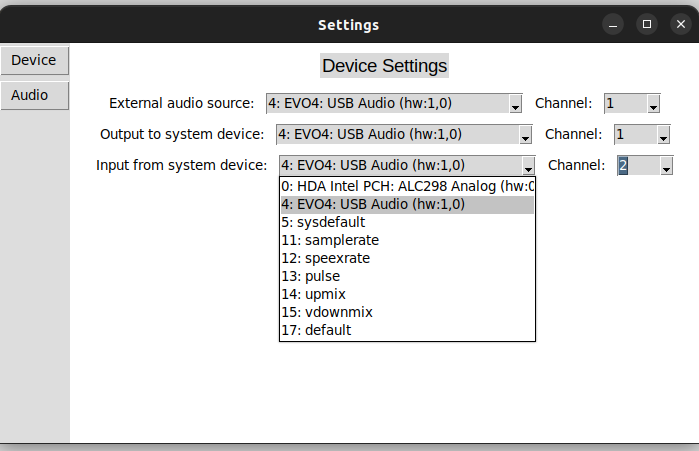
\includegraphics[width=0.6
	\linewidth]{Figures/Coro_Device_settings.png}
	\caption{Device Settings Window recognizing EVO 4 soundcard}
	\label{fig:Coro_device_settings}
\end{figure}

Left default audio settings ............................................................

\begin{figure}[H]
	\centering
	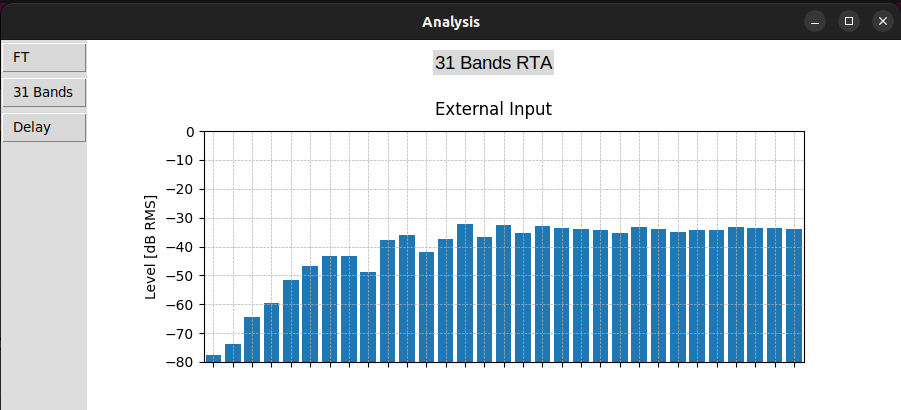
\includegraphics[width=0.6
	\linewidth]{Figures/Coro_Pink_Bad.png}
	\caption{First RTA measurement over the External Input}
	\label{fig:Coro_Bad_Pink}
\end{figure}

\begin{figure}[H]
	\centering
	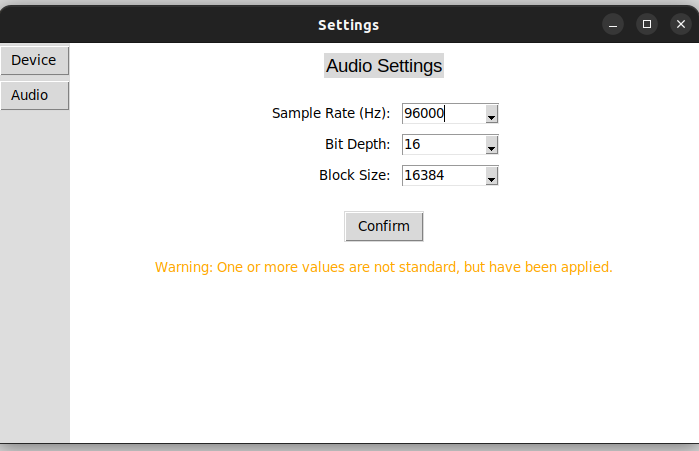
\includegraphics[width=0.6
	\linewidth]{Figures/Coro_audio_settings.png}
	\caption{Audio Settings Window after changes}
	\label{fig:Coro_audio_settings}
\end{figure}

Bloc Size too small --> Change BlockSize to 16384 --> 96KHz = 170.7ms ...........................................

\begin{figure}[H]
	\centering
	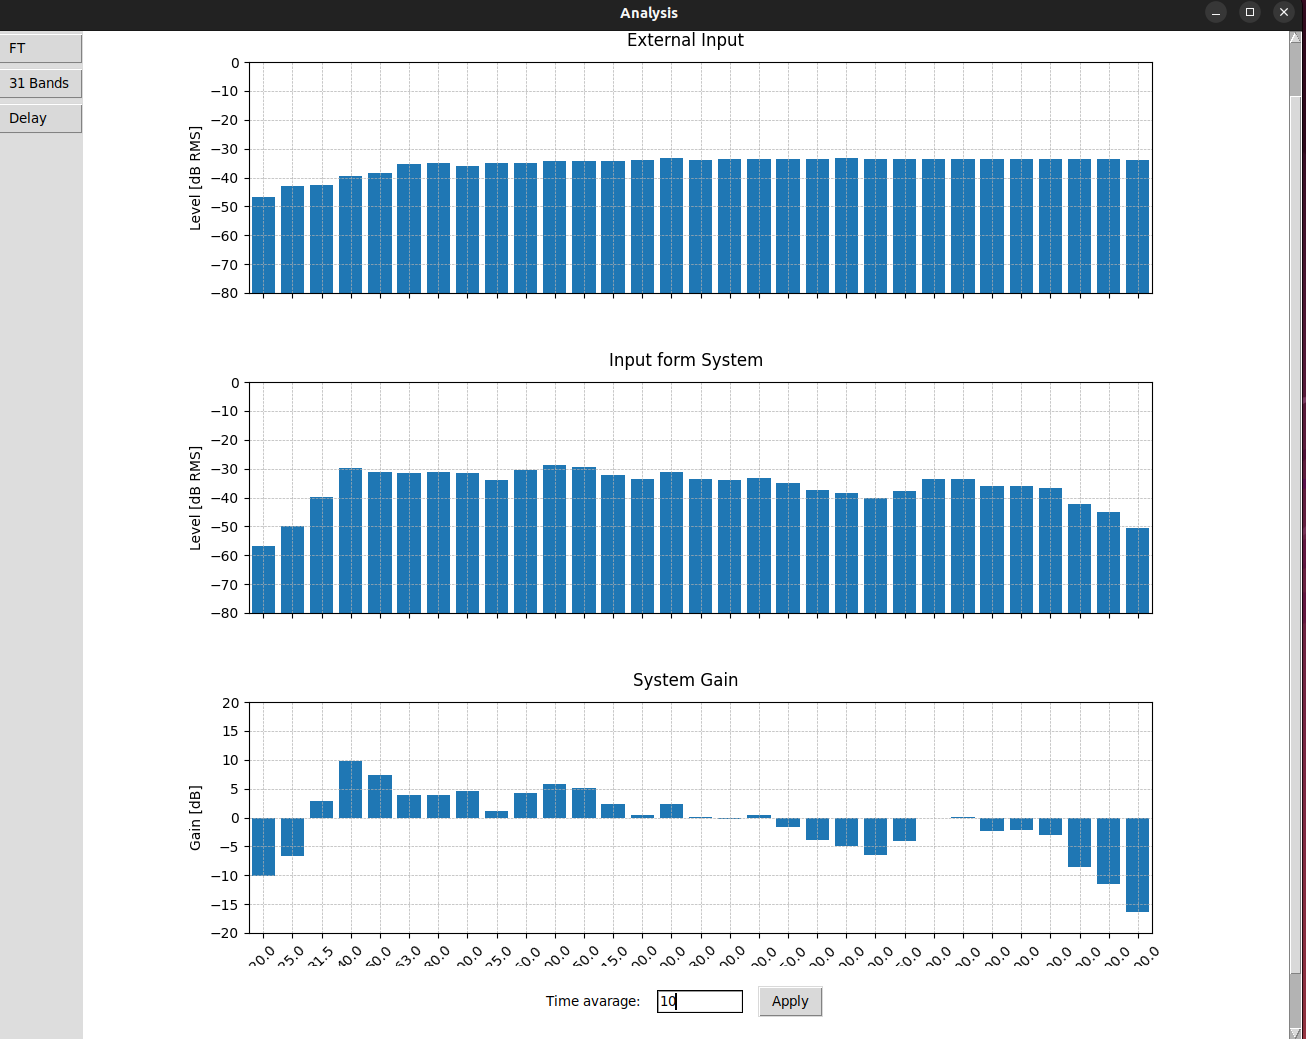
\includegraphics[width=0.6
	\linewidth]{Figures/Coro_Pink_Good.png}
	\caption{Second delay measurement..............................................................}
	\label{fig:Coro_Good_Pink}
\end{figure}

\begin{figure}[H]
	\centering
	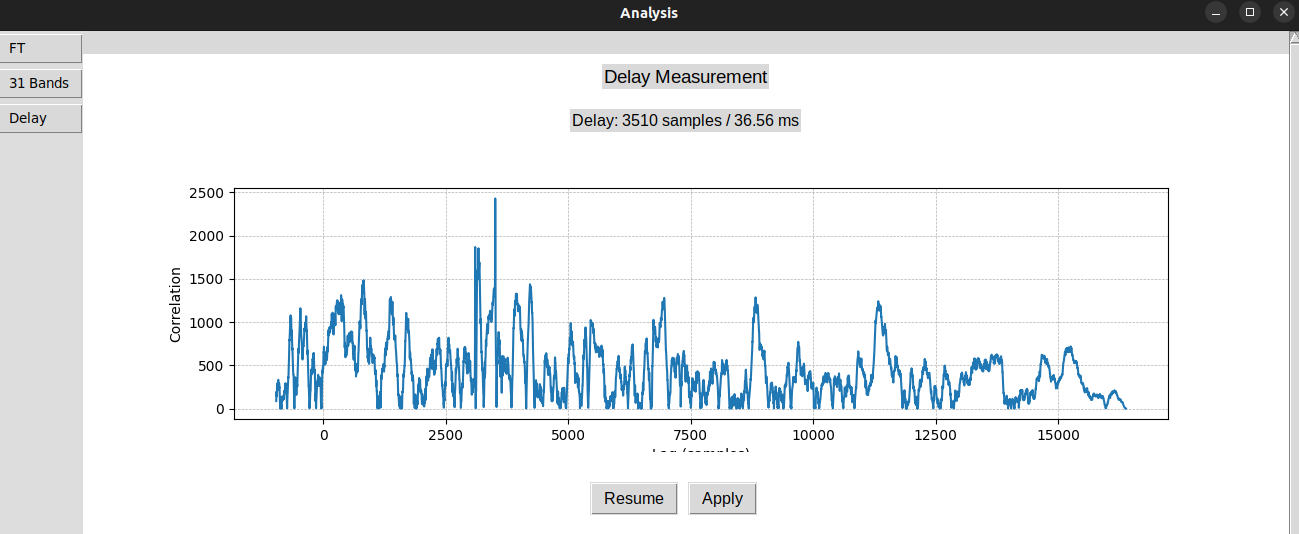
\includegraphics[width=0.6
	\linewidth]{Figures/Coro_Delay.png}
	\caption{First delay measurement...............................................................}
	\label{fig:Coro_delay1}
\end{figure}

36.56ms = 12.43m (340m/s) .........................................................................

\begin{figure}[H]
	\centering
	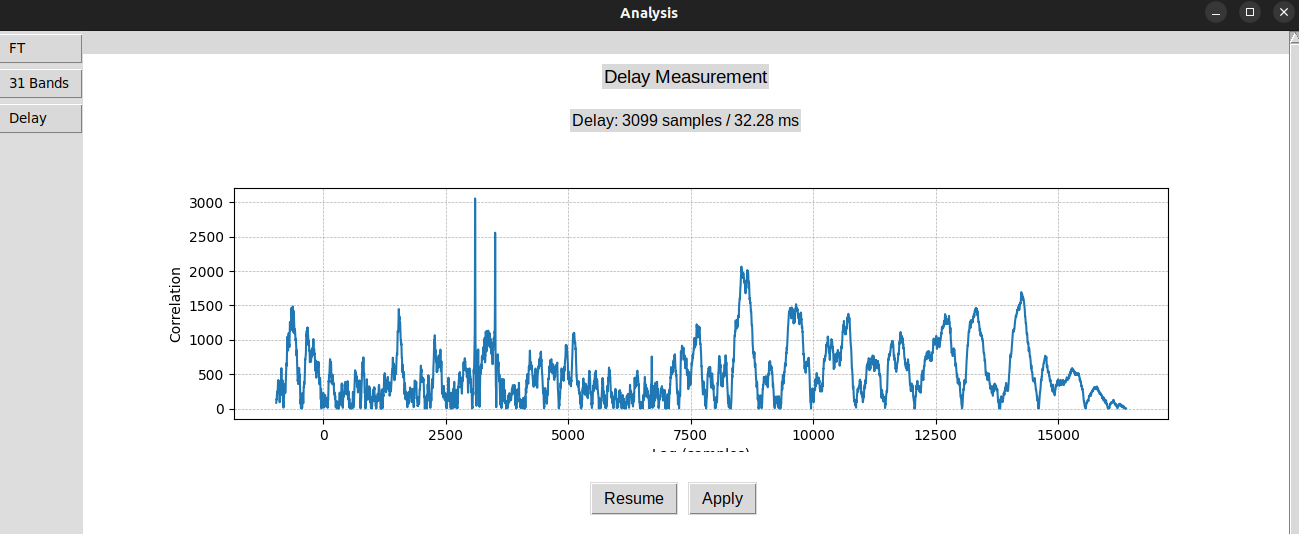
\includegraphics[width=0.6
	\linewidth]{Figures/Coro_delay_2.png}
	\caption{Second delay measurement..............................................................}
	\label{fig:Coro_delay2}
\end{figure}

32.28ms = 10.98m (340m/s) ..............................................................

\begin{figure}[H]
	\centering
	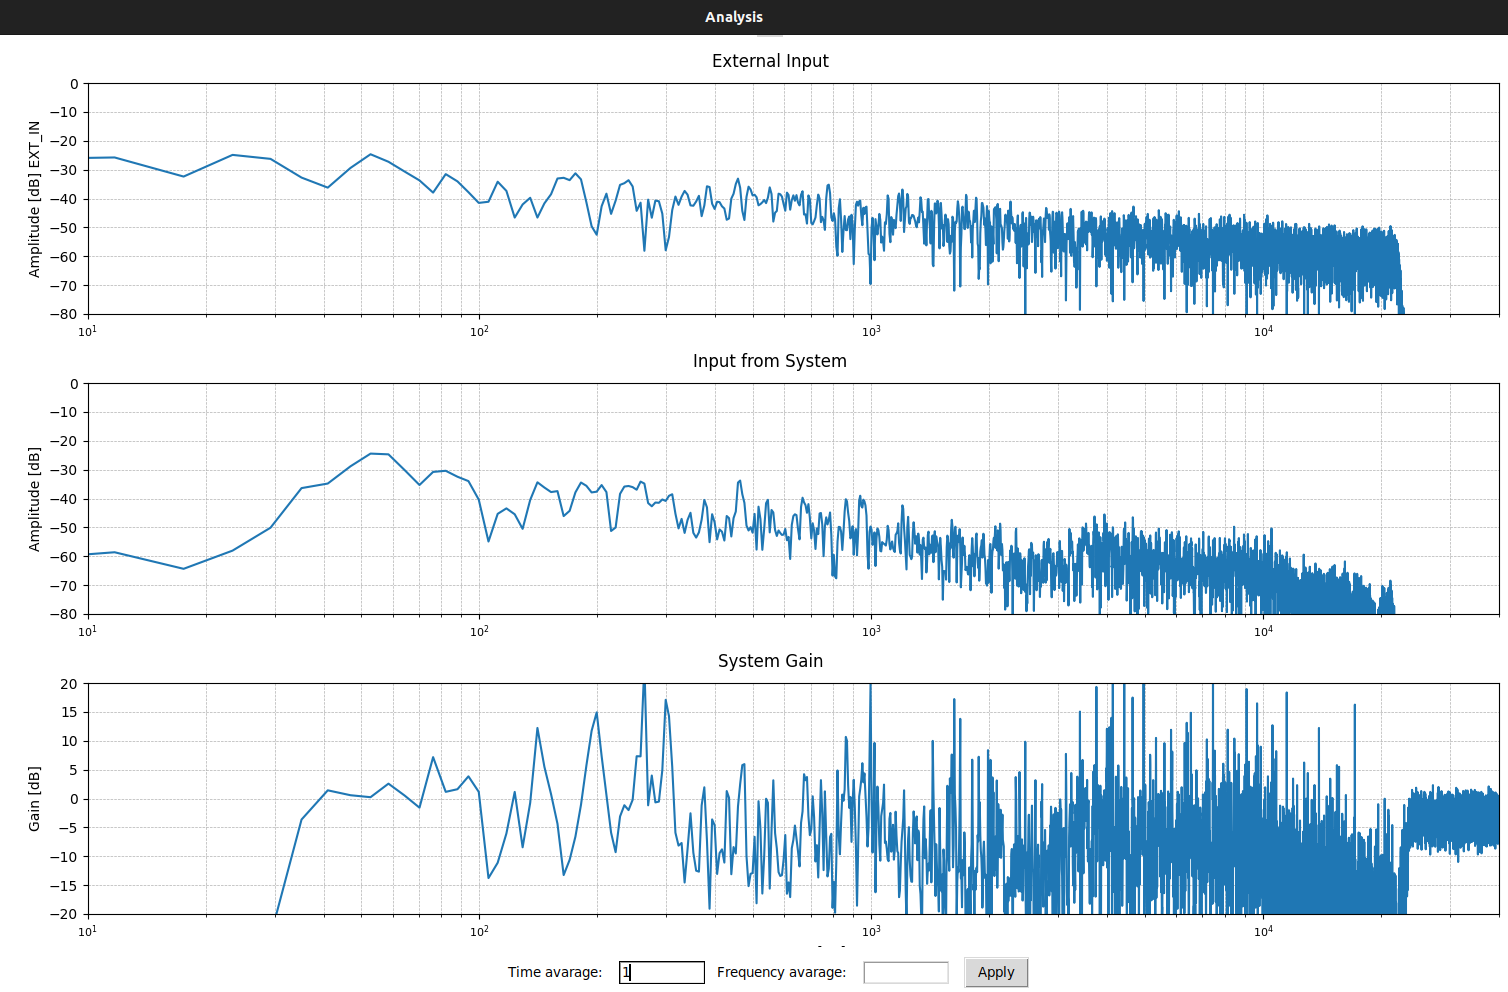
\includegraphics[width=0.6
	\linewidth]{Figures/Coro_FT_NO_av.png}
	\caption{FT - Pink Noise - No Avarage..............................................................}
	\label{fig:Coro_FT_no_av}
\end{figure}

\begin{figure}[H]
	\centering
	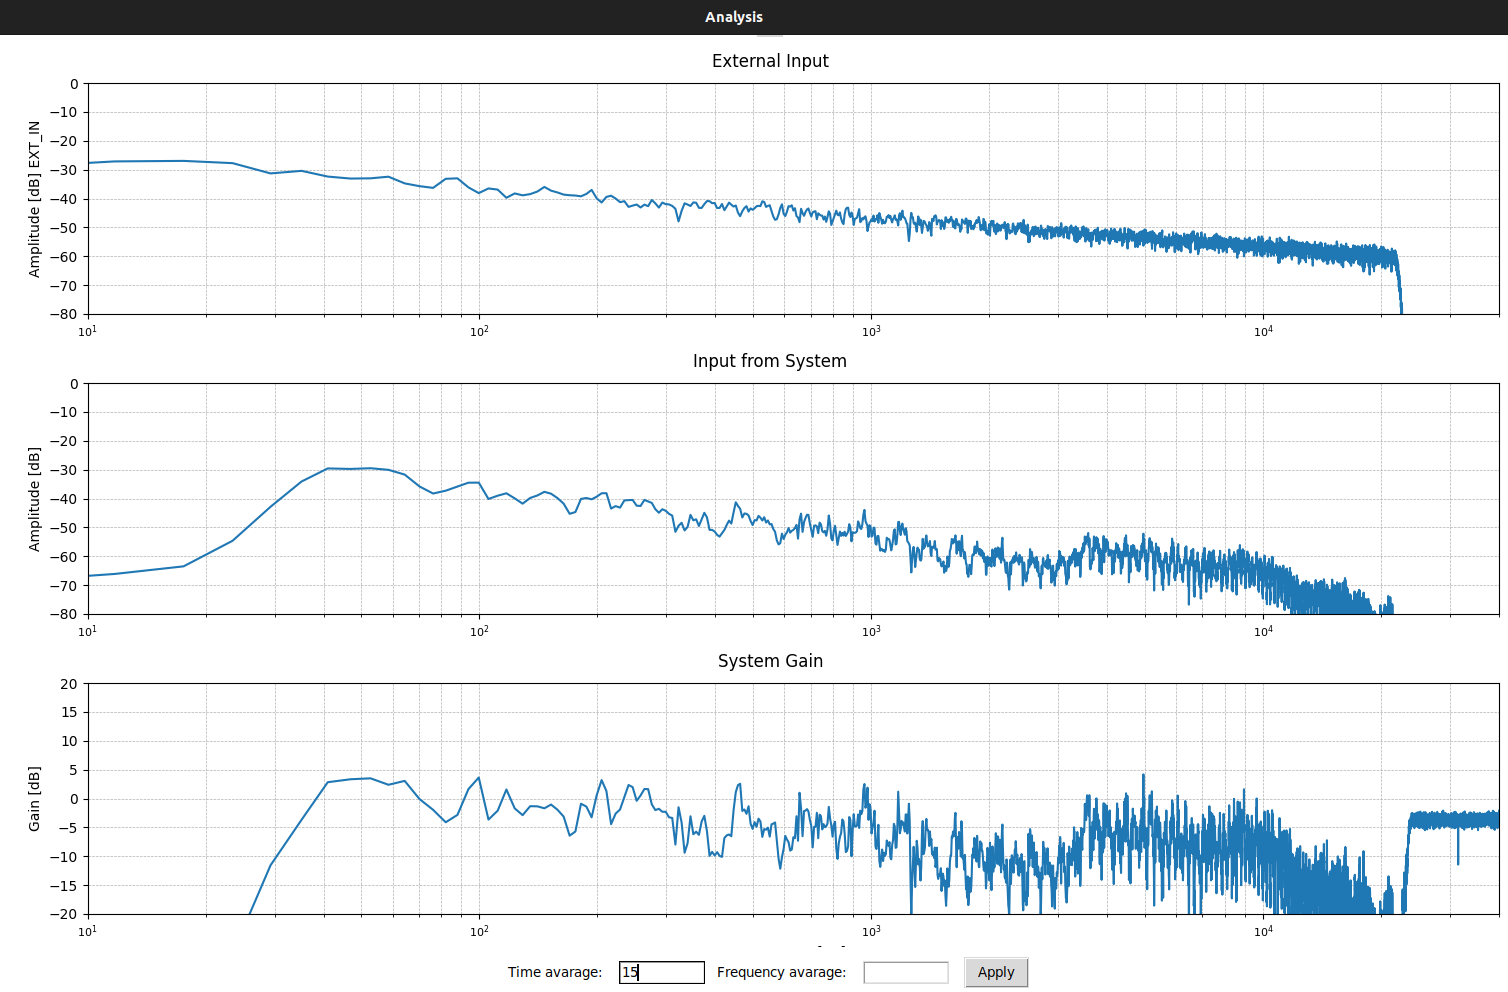
\includegraphics[width=0.6
	\linewidth]{Figures/Coro_FT_time_av.png}
	\caption{FT - Pink Noise - Time Avarage..............................................................}
	\label{fig:Coro_FT_time_av}
\end{figure}

\begin{figure}[H]
	\centering
	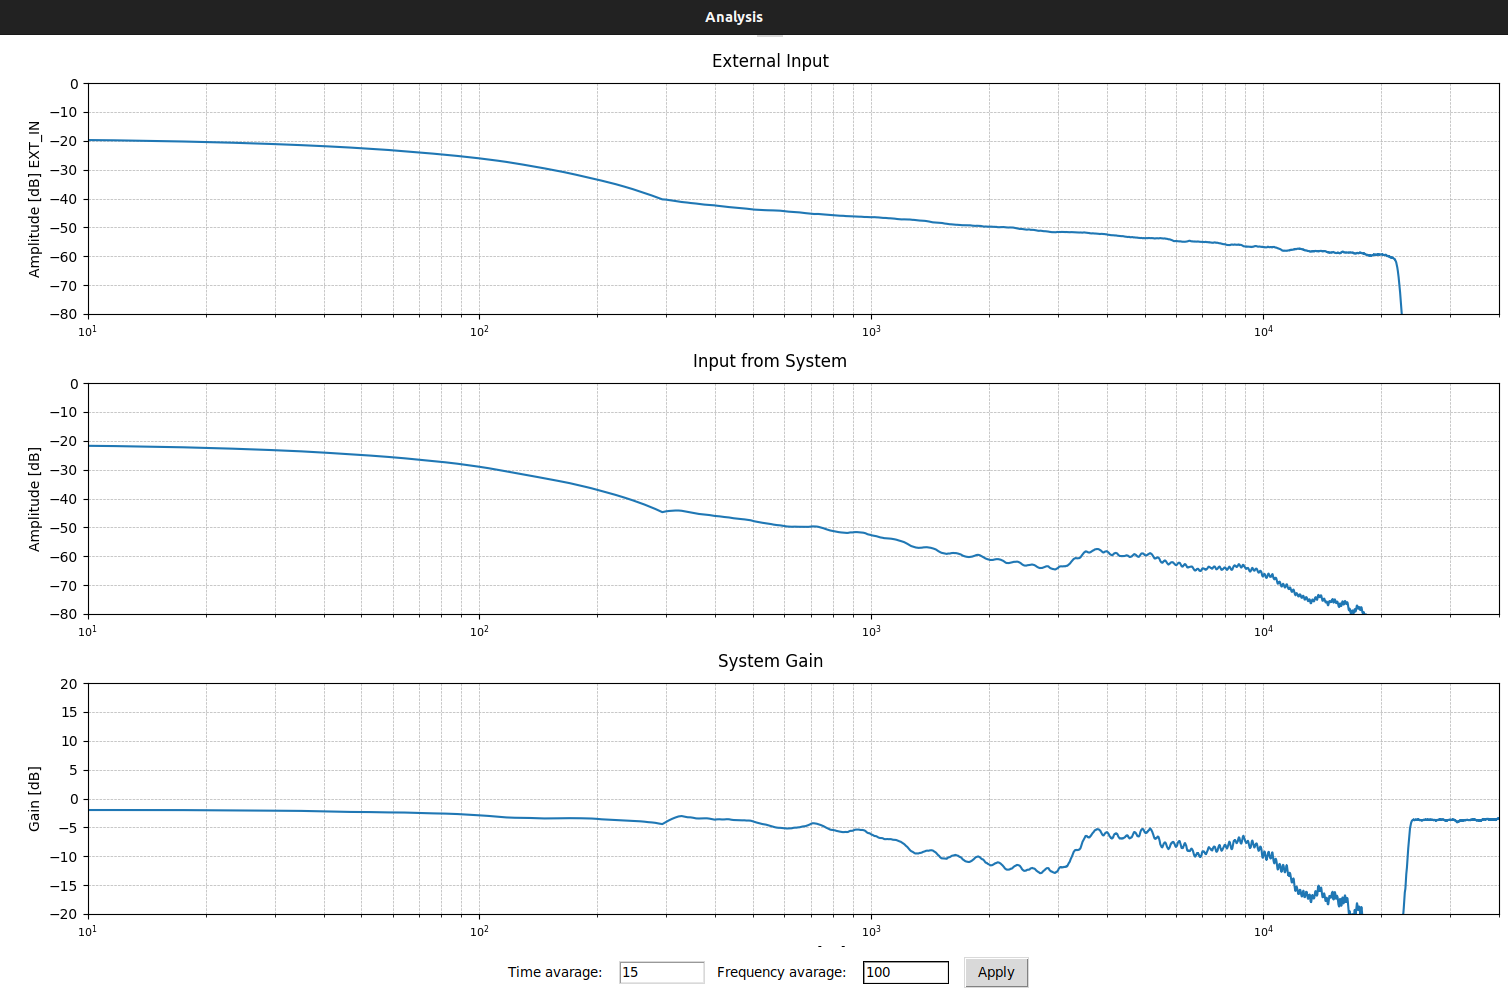
\includegraphics[width=0.6
	\linewidth]{Figures/Coro_FT_WITH_av.png}
	\caption{FT - Pink Noise - Time Avarage + Frequency Average...........................................}
	\label{fig:Coro_FT_av}
\end{figure}

\begin{figure}[H]
	\centering
	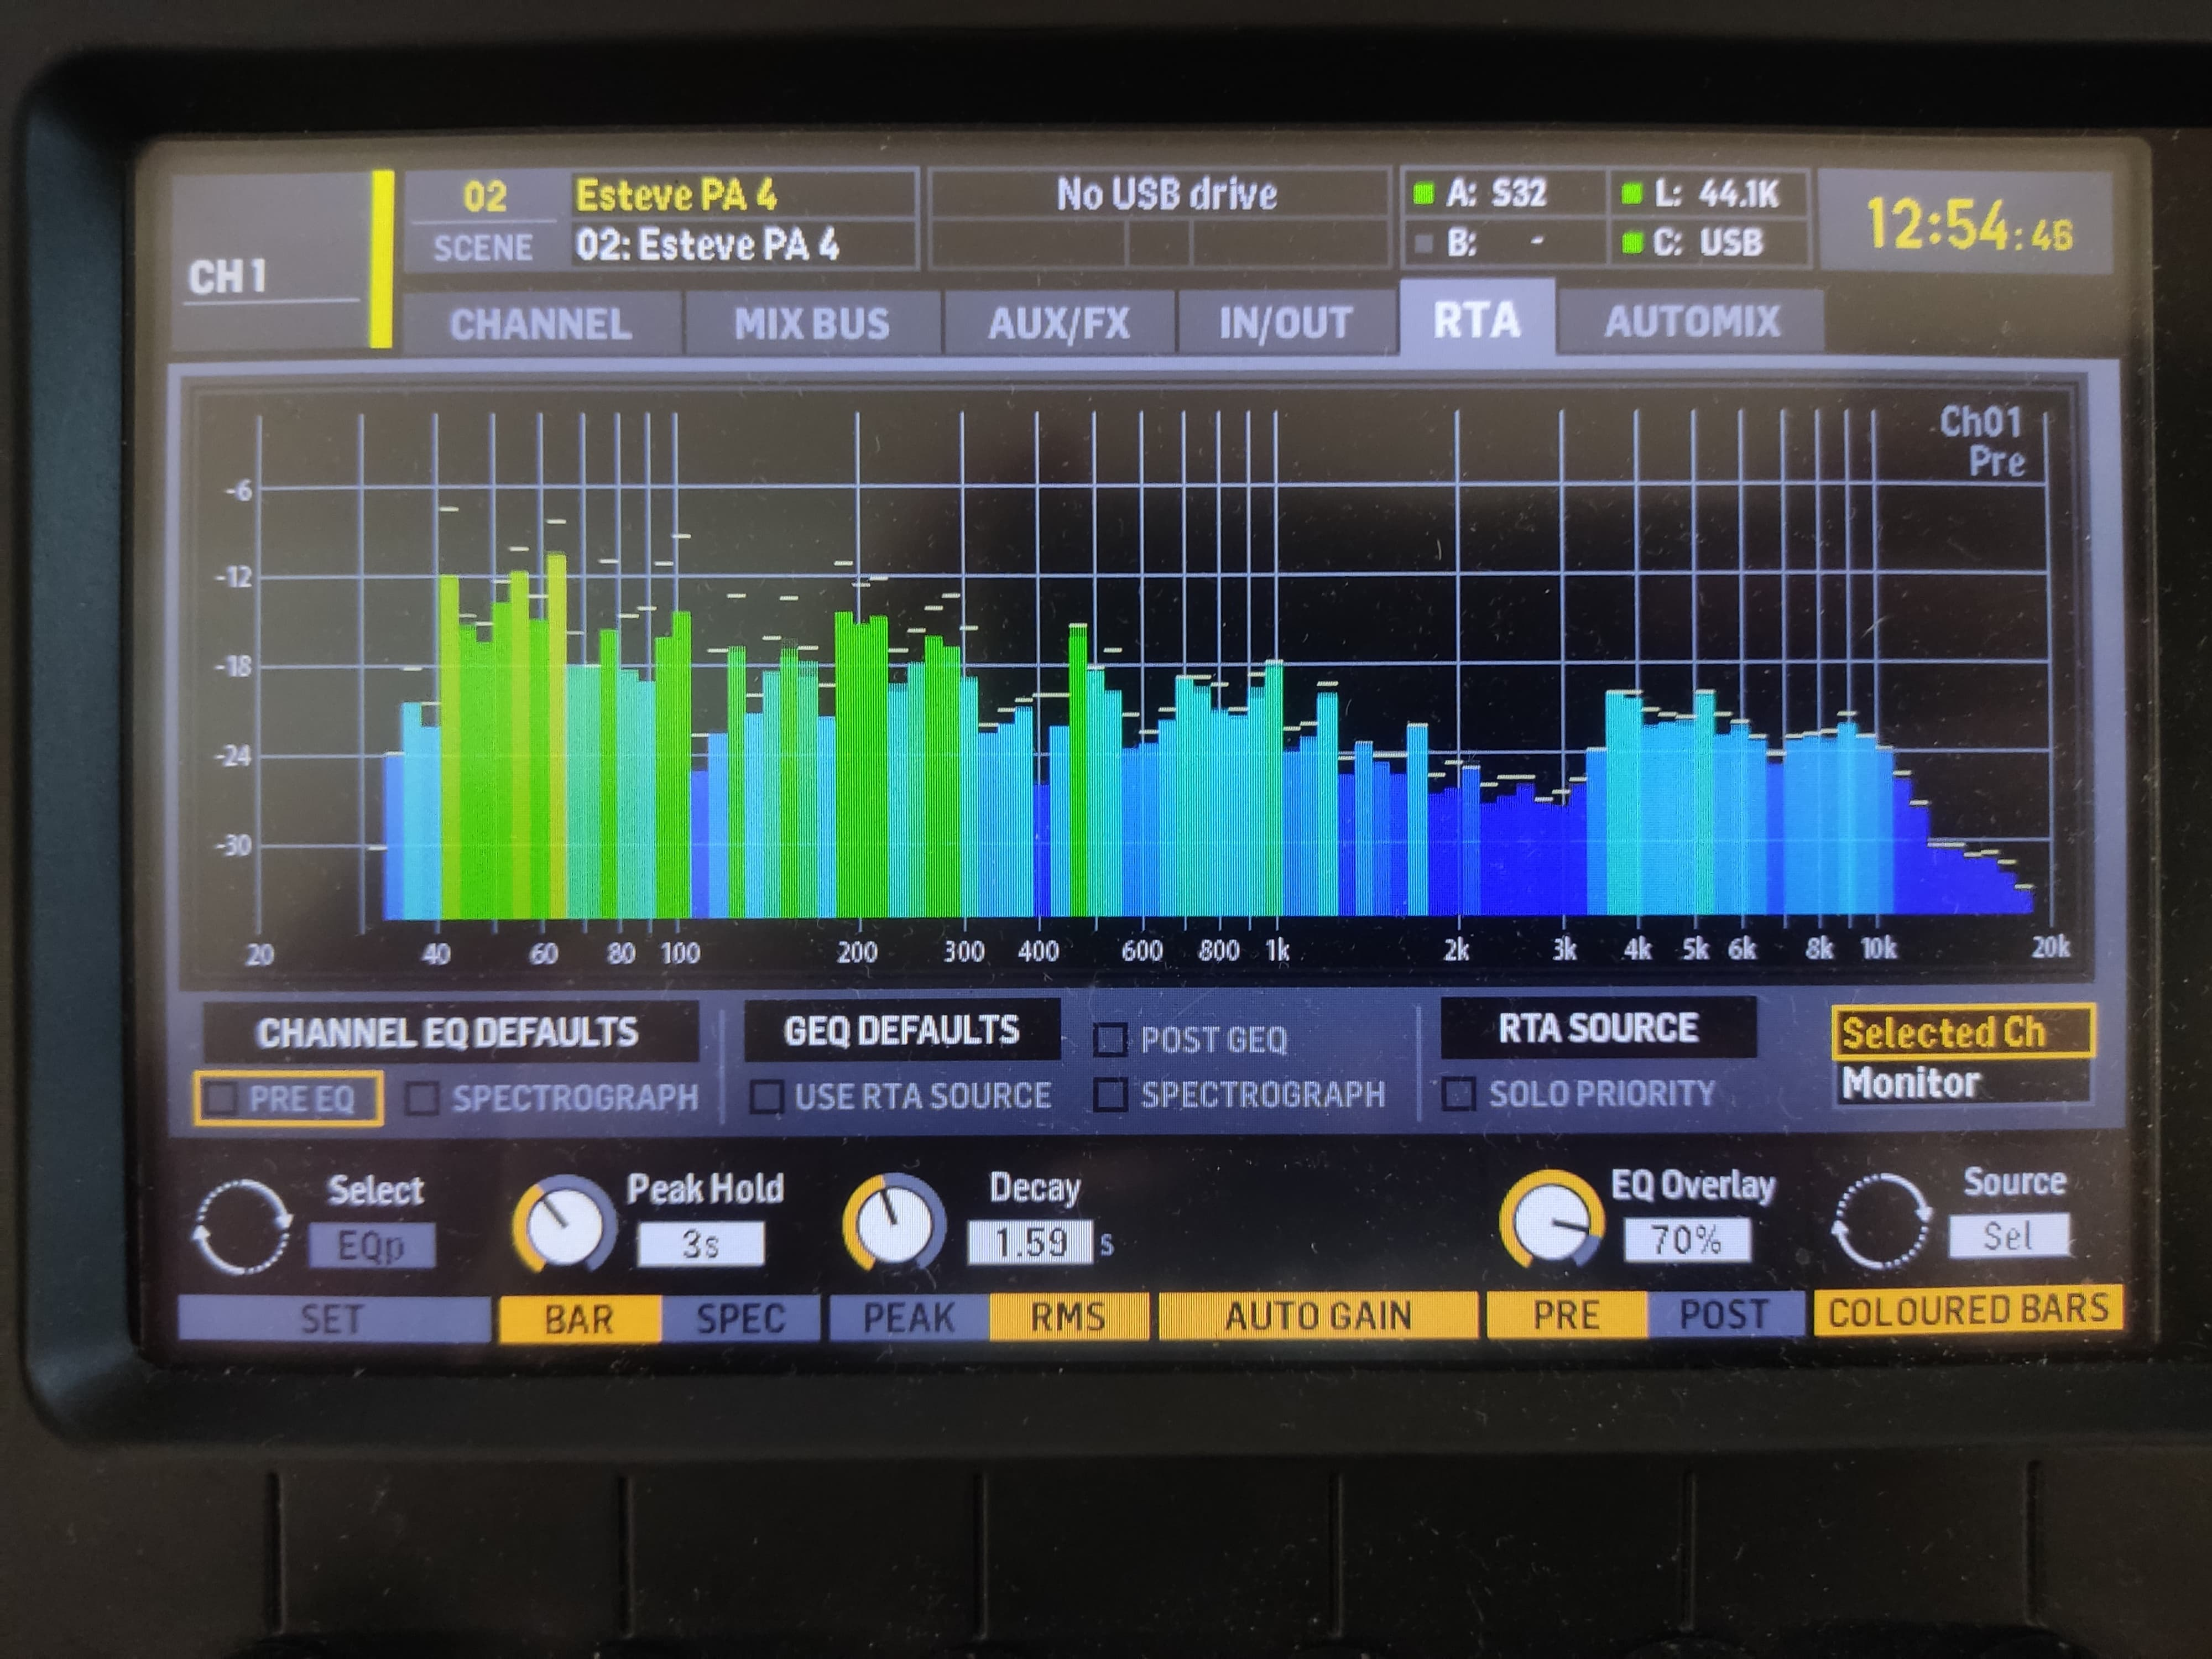
\includegraphics[width=0.6
	\linewidth]{Figures/Coro_X32_nontreated.jpeg}
	\caption{Microphone caption without any treatment, using X32 analysis tool....................}
	\label{fig:Coro_X32_nontreated}
\end{figure}

\begin{figure}[H]
	\centering
	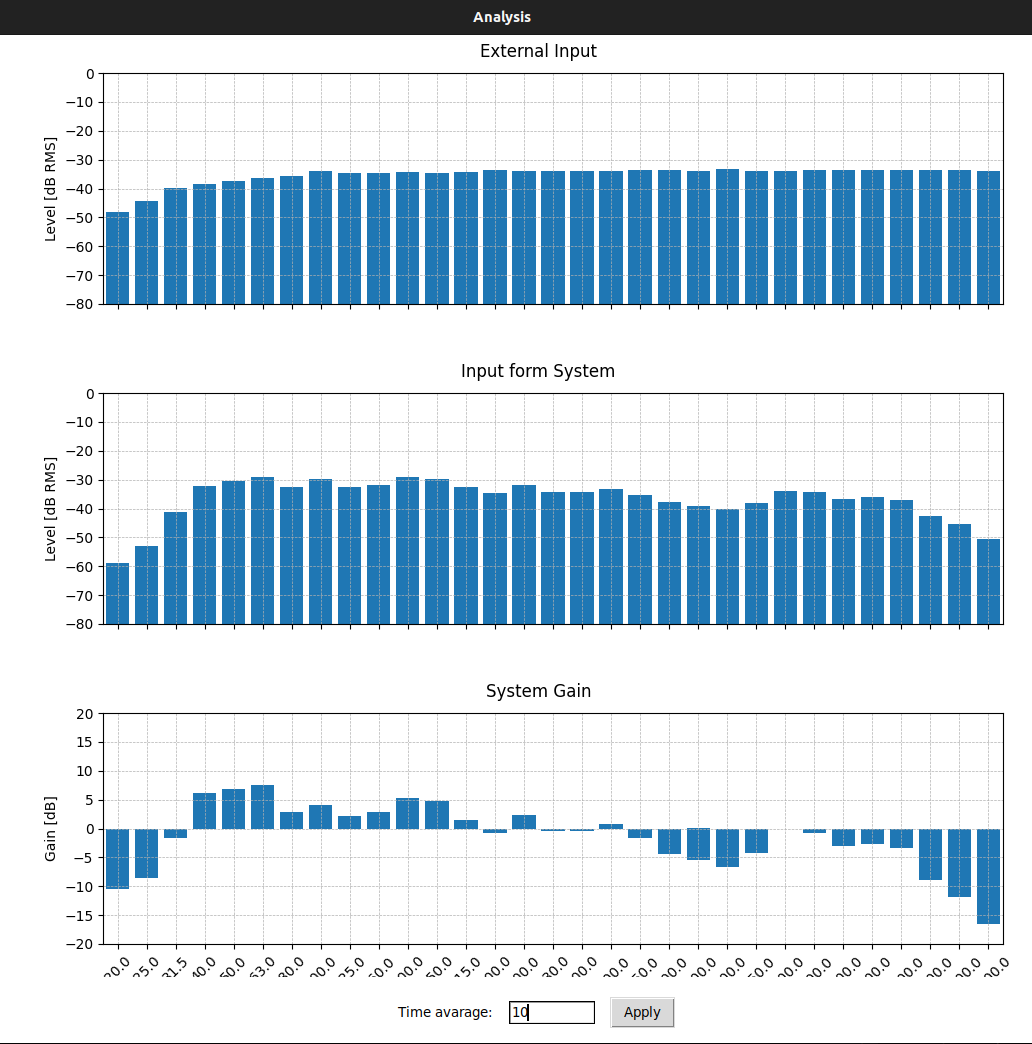
\includegraphics[width=0.6
	\linewidth]{Figures/Coro_RTA_Saved.png}
	\caption{Non treated Pink Noise, Saved results..............................................................}
	\label{fig:Coro_RTA_saved}
\end{figure}

\begin{figure}[H]
	\centering
	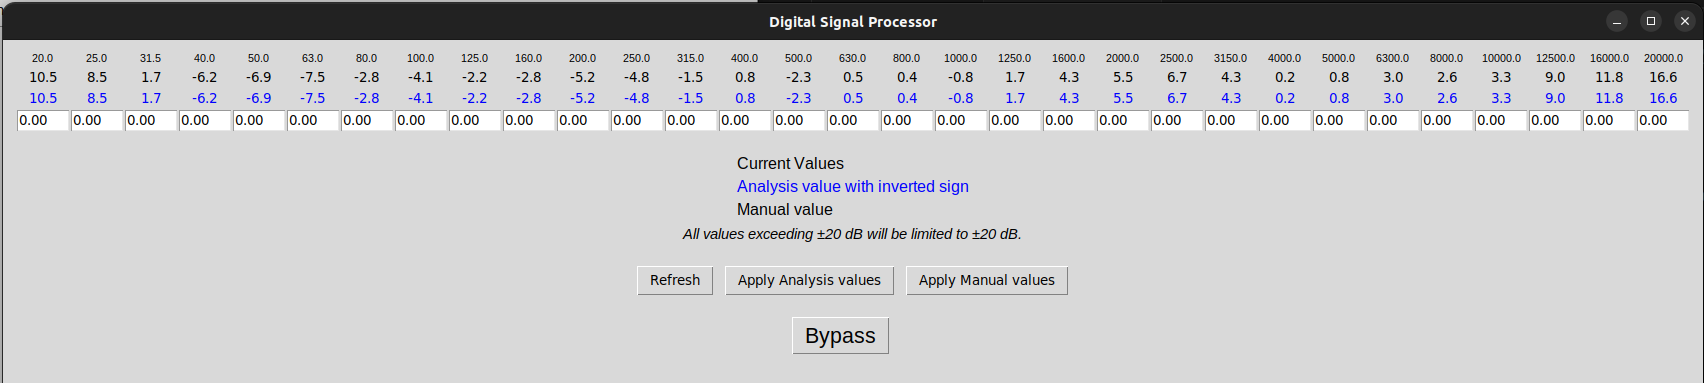
\includegraphics[width=1
	\linewidth]{Figures/Coro_EQ_from_RTA.png}
	\caption{EQ values applyed form RTA analysis..............................................................}
	\label{fig:Coro_EQ_RTA+C}
\end{figure}

\begin{figure}[H]
	\centering
	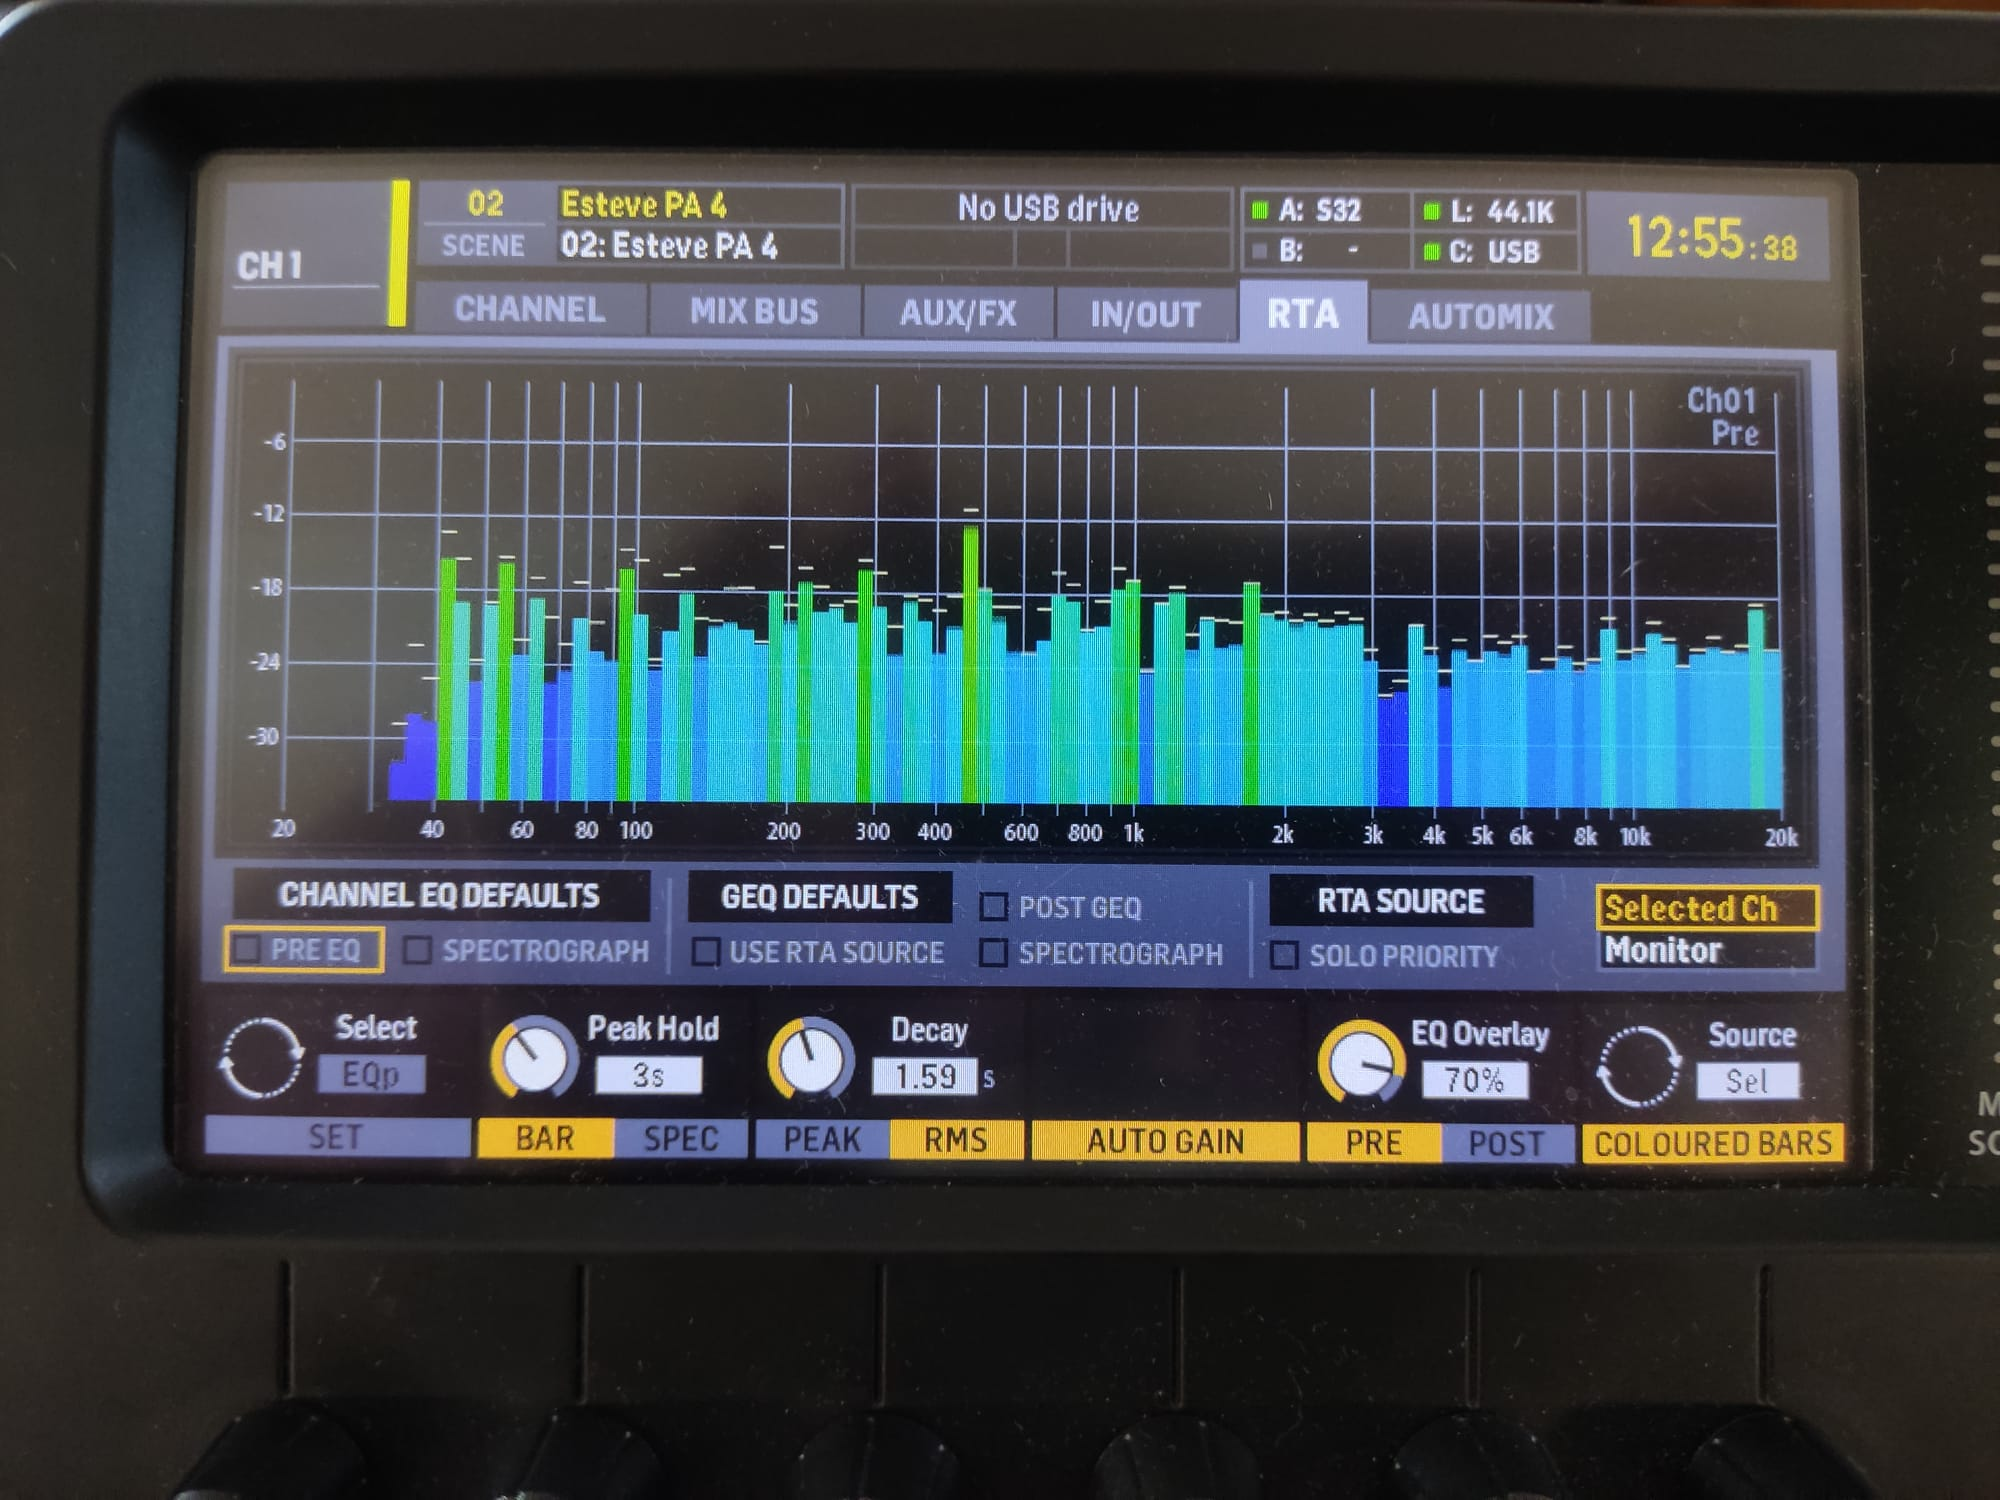
\includegraphics[width=0.6
	\linewidth]{Figures/Coro_X32_treatedRTAc.jpeg}
	\caption{Microphone caption with treatment by RTA+C, using X32 analysis tool..................}
	\label{fig:Coro_X32_RTA+C}
\end{figure}

\begin{figure}[H]
	\centering
	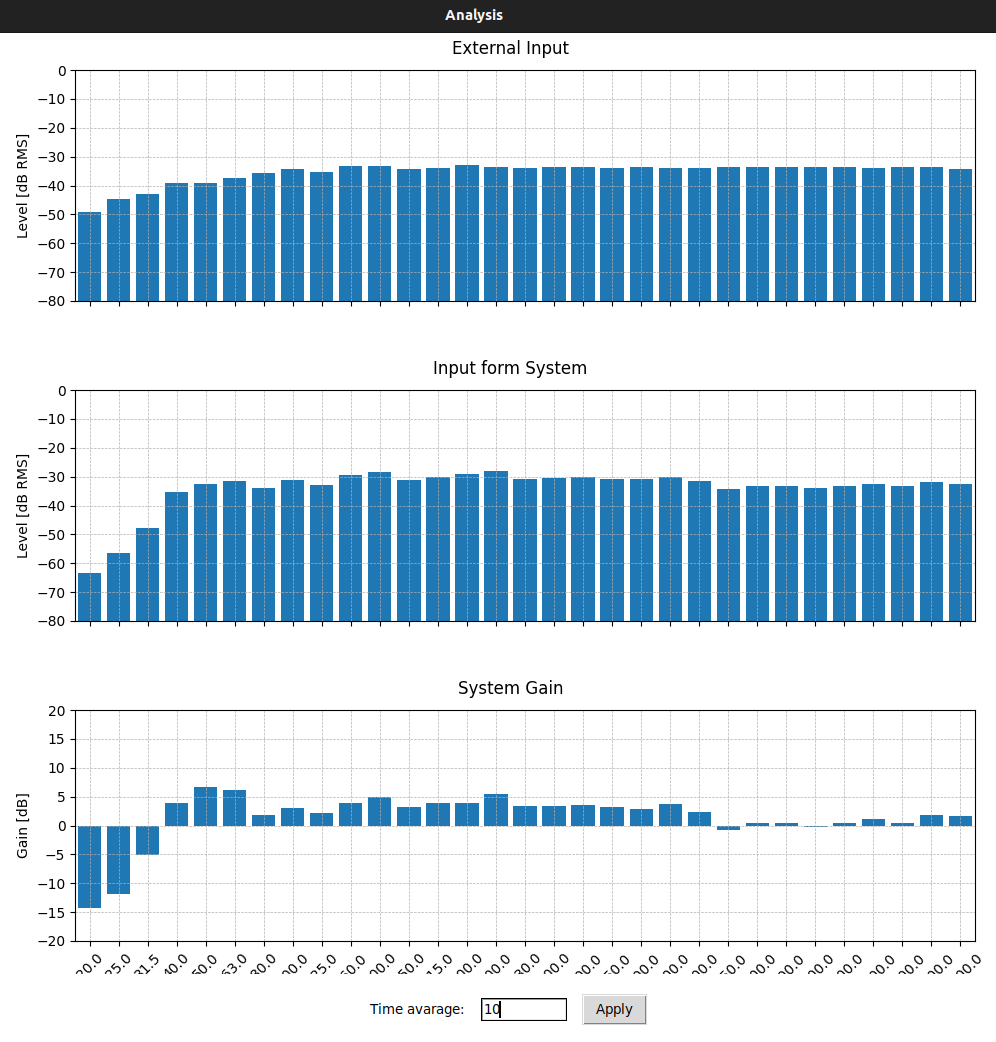
\includegraphics[width=0.6
	\linewidth]{Figures/Coro_RTA+EQ_ON.png}
	\caption{Pink Noise with processed signal by RTA+C program..............................................................}
	\label{fig:Coro_RTA_RTA+C}
\end{figure}

\begin{figure}[H]
	\centering
	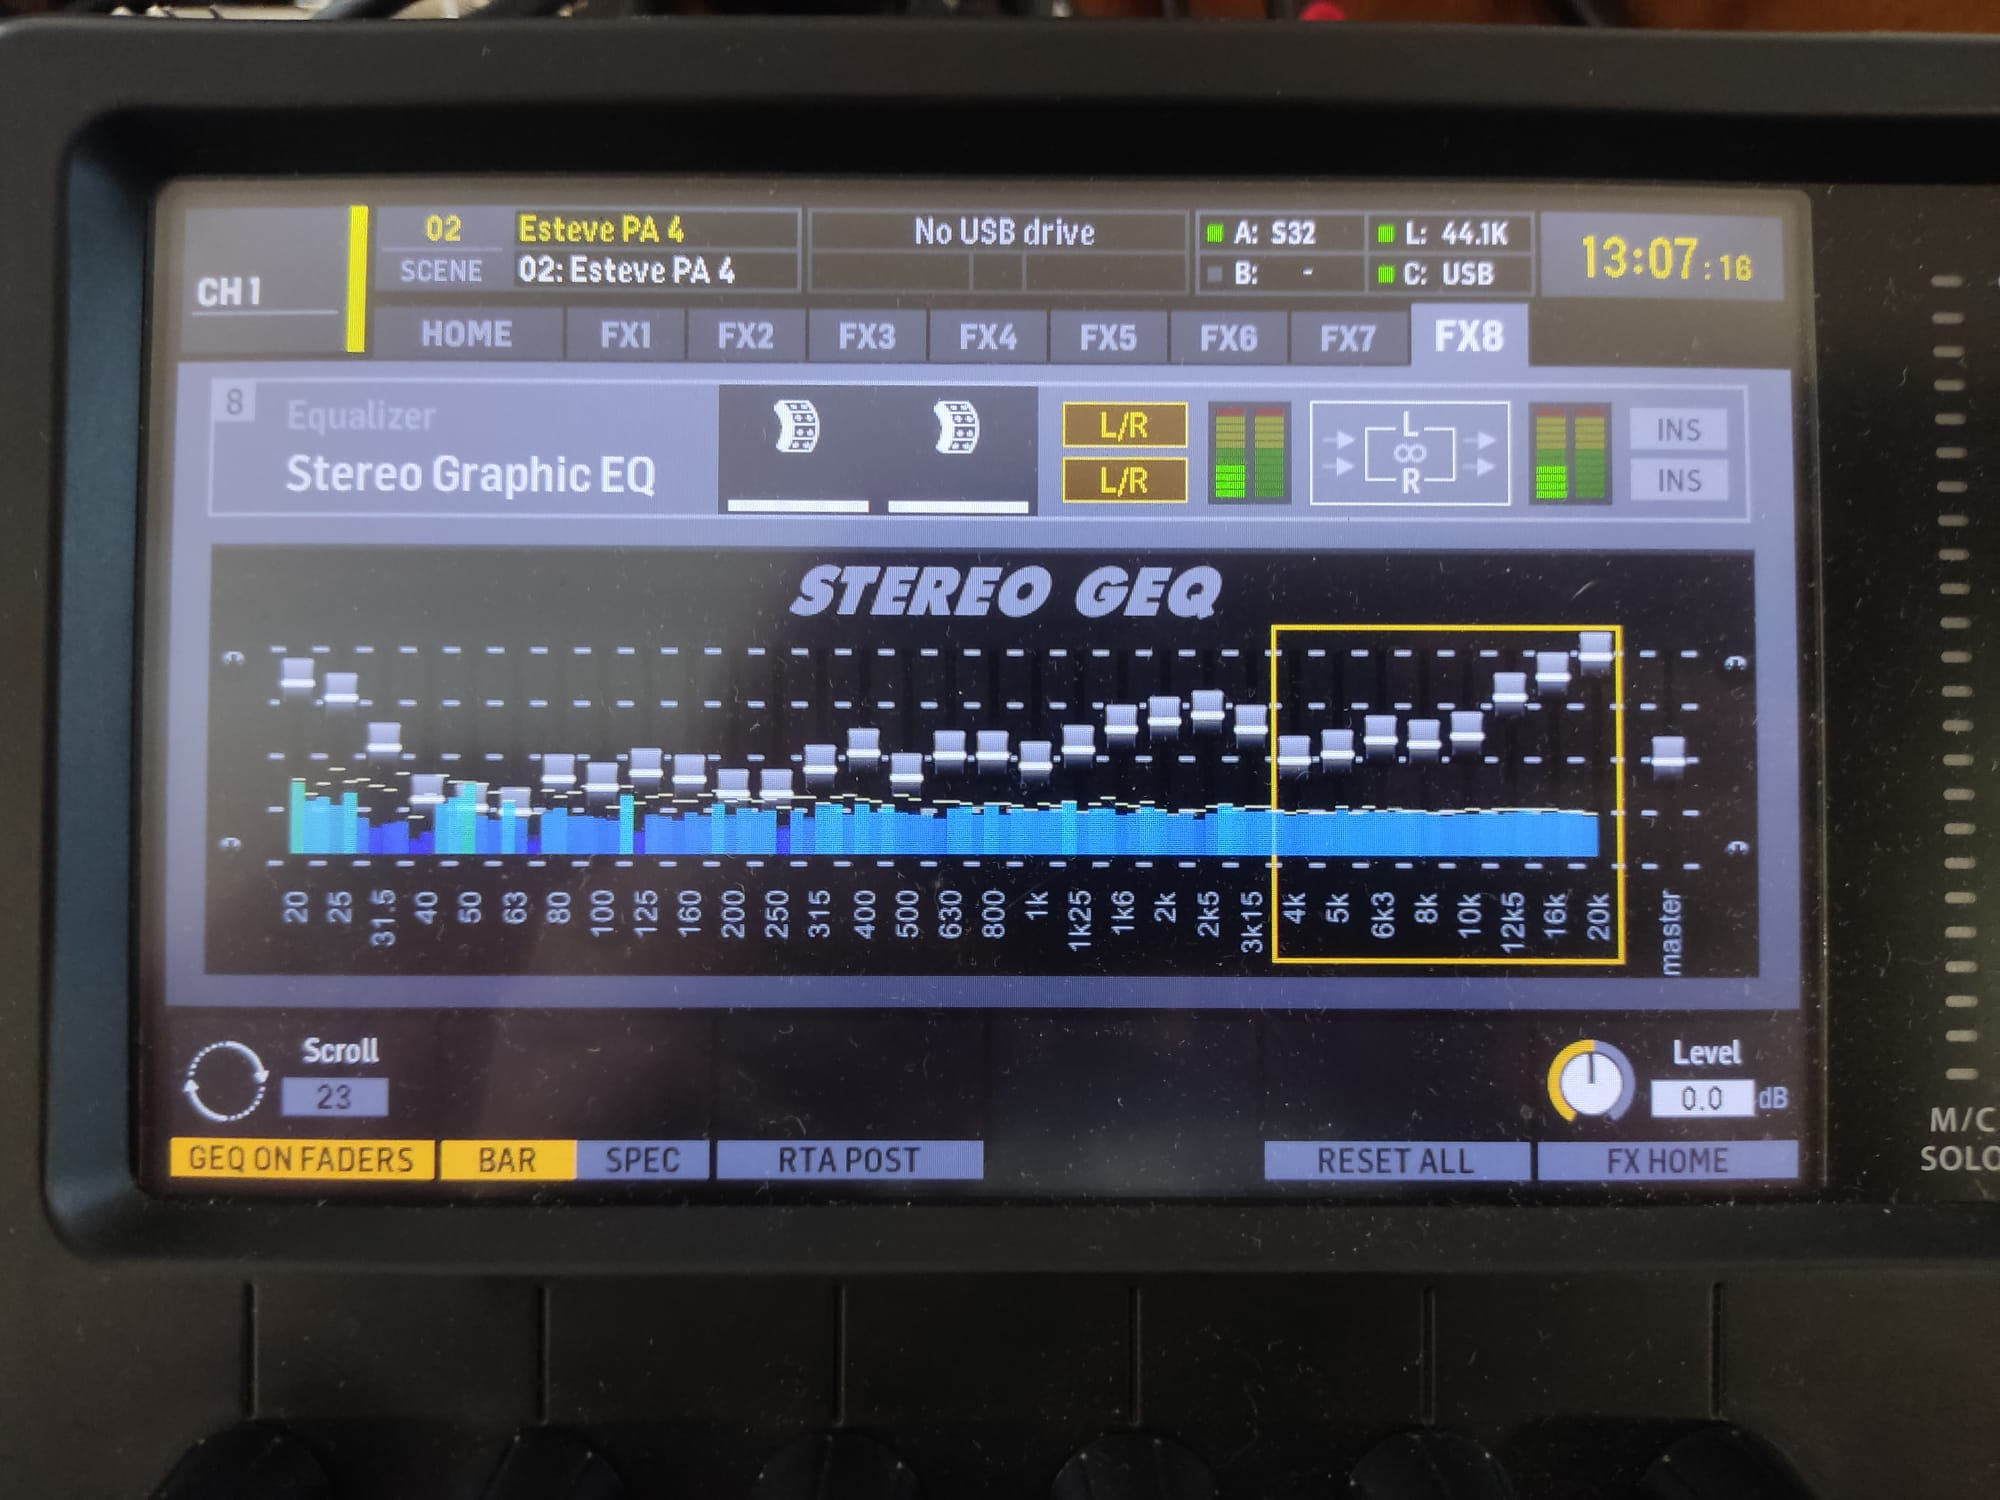
\includegraphics[width=0.6
	\linewidth]{Figures/Coro_X32_EQ.jpeg}
	\caption{Setting X32 EQ tool with parameters of RTA+C ........................................}
	\label{fig:Coro_X32_EQ}
\end{figure}

\begin{figure}[H]
	\centering
	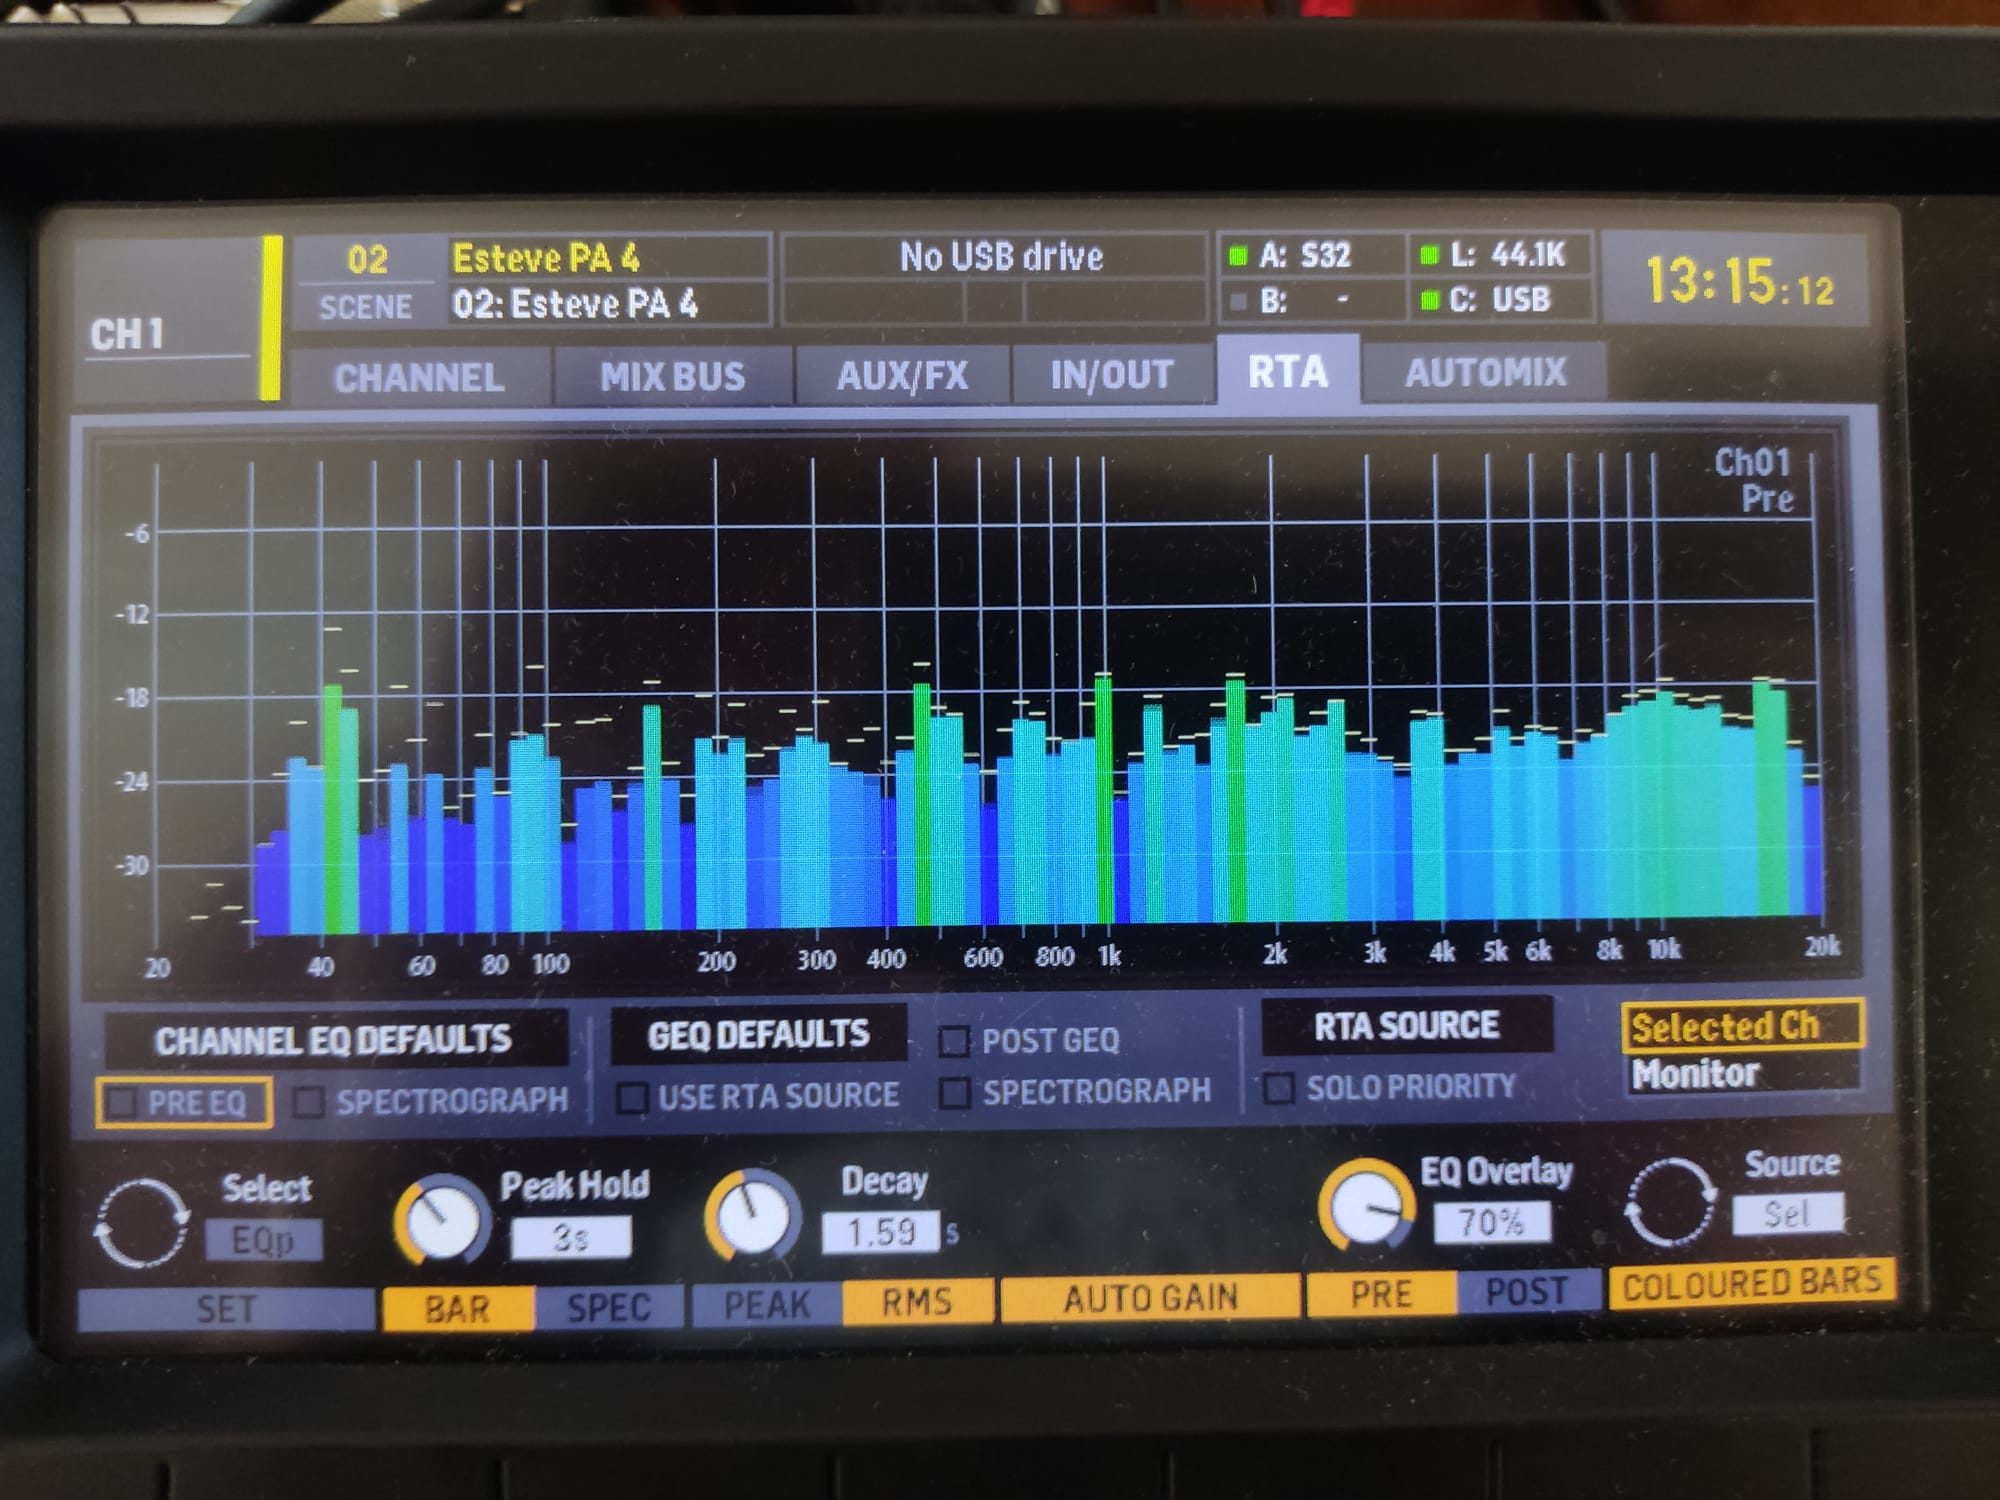
\includegraphics[width=0.6
	\linewidth]{Figures/Coro_X32_treatedX32.jpeg}
	\caption{Microphone caption with treatment of X32-EQ tool and using X32 analysis tool.........}
	\label{fig:Coro_X32_treatedX32}
\end{figure}

For music, use X32 EQ becouse the glitch ....................................................................

\begin{figure}[H]
	\centering
	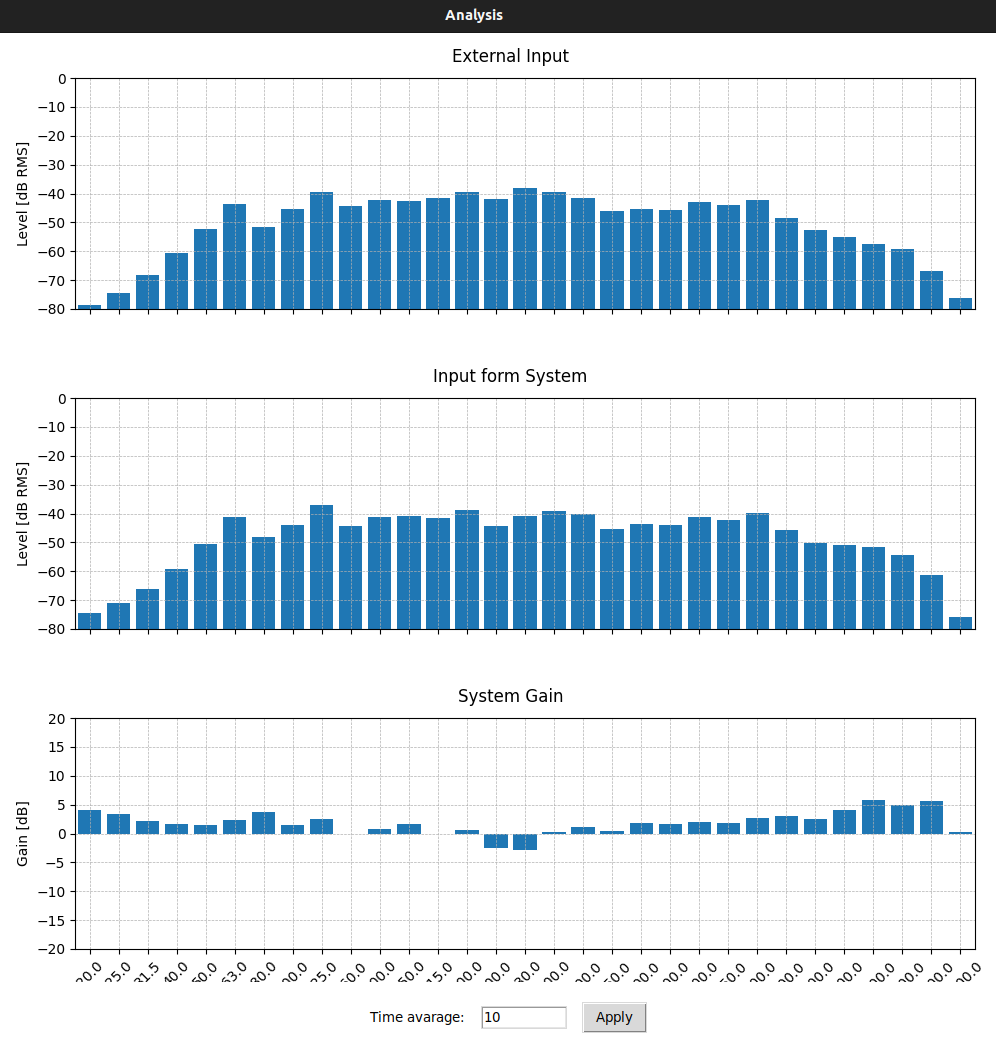
\includegraphics[width=0.6
	\linewidth]{Figures/Coro_Music_EQ_X32.png}
	\caption{RTA, using music, and EQ from X32..............................................................}
	\label{fig:Coro_RTA_music}
\end{figure}

\begin{figure}[H]
	\centering
	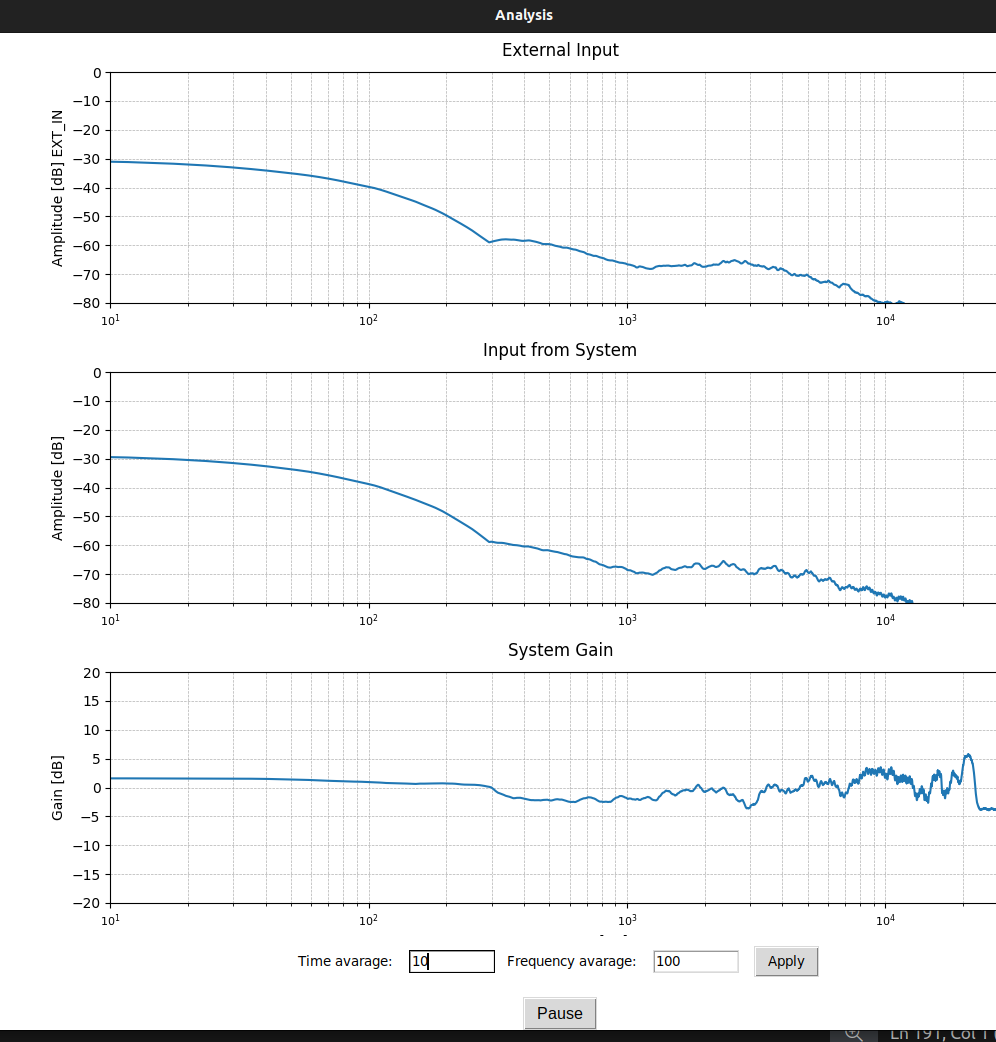
\includegraphics[width=0.6
	\linewidth]{Figures/Coro_FT_music_EQX32.png}
	\caption{FT, using music, and EQ from X32..............................................................}
	\label{fig:Coro_FT_music}
\end{figure}

Looks preaty nice .......................................................................

